% !TEX program = xelatex
% 华数杯数学建模竞赛论文骨架。
% 依据 format2024.doc：电子版从摘要专用页开始，摘要页计为第 1 页；
% 正文紧随其后，不设置纸质承诺书、编号专用页或正文目录。
\documentclass[fontset=windows,a4paper]{ctexart}

\usepackage[a4paper,margin=2.5cm]{geometry}
\usepackage{amsmath,amssymb}
\usepackage{booktabs,array,longtable}
\usepackage{graphicx,float}
\usepackage{caption}
\usepackage{fancyhdr}
\usepackage{enumitem}
\usepackage{xcolor}
\usepackage{listings}
\usepackage[unicode]{hyperref}

% 严格复刻 CUMCM-2025B 优秀范文的正文密度：使用 ctexart 默认字号和默认基线，
% 不额外设置 12pt、\linespread 或西文字体覆盖。
\setlength{\parindent}{2em}
\setlength{\parskip}{0pt}
\setcounter{secnumdepth}{3}
\setcounter{tocdepth}{3}

% 图表标题、页眉页脚与优秀范文保持一致。
\captionsetup{labelsep=space,font=small,justification=centering}
\pagestyle{fancy}
\fancyhf{}
\fancyfoot[C]{\thepage}
\renewcommand{\headrulewidth}{0pt}
\hypersetup{colorlinks=true,linkcolor=black,citecolor=black,urlcolor=black}

\lstset{
  basicstyle=\ttfamily\small,
  frame=single,
  breaklines=true,
  showstringspaces=false,
  columns=fullflexible,
  keepspaces=true,
}

\begin{document}
\pagenumbering{arabic}
\setcounter{page}{1}

% ==================== 摘要专用页 ====================
\begin{center}
  \vspace*{0.2cm}
  {\Large\bfseries VLSI 布图规划的几何建模与优化求解}
  \vspace*{1cm}

  {\Large\bfseries 摘\quad 要}
\end{center}
\thispagestyle{fancy}

本文针对超大规模集成电路硬模块的布图规划问题，建立了统一描述模块旋转、几何非重叠、芯片轮廓与互连线长的分层组合优化模型。我们分别面向自由轮廓面积优化、固定轮廓线长优化、死区率压缩和非矩形模块推广，设计了矩形装箱构造、目标引导合法化、整数边长搜索与形状级精确枚举算法。通过对三组规模化网表和非矩形算例进行求解与约束复核，我们成功得到各阶段的可行布局、轮廓参数及线长结果，并基于结果揭示了轮廓面积、布局形状与互连线长之间的制约关系，以及形状级建模对利用非矩形模块凹槽空间的作用。

\noindent\textbf{针对问题一、}为最小化允许 $90^\circ$ 旋转的硬模块自由轮廓面积，我们建立了\textbf{可旋转二维矩形装箱模型}，以外接面积最小为主目标，并在同面积时进一步优化轮廓长短边比。针对轮廓尺度未知且组合空间庞大的问题，以候选短边搜索轮廓尺寸，并结合\textbf{Skyline 与 MaxRects}构造布局。\texttt{n100}、\texttt{n200}、\texttt{n300} 三组算例的外接面积分别为 $185330$、$180900$、$289640$；前两组面积冗余率仅为\textbf{3.2473\%、2.9619\%}，但长短边比达到 $25.0581$、$50.2500$，第三组冗余率为 $6.0292\%$、长短边比则降至 $1.0712$，表明自由轮廓下\textbf{面积紧凑性与轮廓均衡性存在竞争关系}。

\noindent\textbf{针对问题二、}在死区率为 $0.15$ 的固定正方形轮廓内，以总半周长线长（HPWL）最小为目标，建立同时考虑模块旋转、边界约束与非重叠约束的布局优化模型。针对离散几何约束与网络线长耦合导致直接联合搜索困难的问题，首先暂时忽略非重叠约束，以\textbf{二次线长松弛}求得模块的网络驱动目标位置；随后采用\textbf{目标引导合法化与局部重插入}：结合目标位置与局部网络信息完成几何合法化，并通过多组模块顺序与插入策略构造候选布局，以降低单一初值的影响；最后针对合法化造成的线长损失，对高线长贡献模块进行局部重插入，在保持布局可行的前提下进一步优化 HPWL。三组实例所得总 HPWL 分别为\textbf{220279.0、410072.5 和 560492.5}；局部重插入使三组实例 HPWL 均进一步下降，不同初始合法化布局仍表现出明显结果差异，表明初始空间结构对最终线长具有持续影响。

\noindent\textbf{针对问题三、}为进一步压缩芯片死区率，我们将其转化为正方形轮廓整数边长的外层搜索问题，并采用“先压缩轮廓、再优化线长”的词典序目标。首先依据模块总面积与最大模块边长确定搜索下界，结合多种 MaxRects 放置规则逐步搜索可行轮廓；随后在所得首个可行边长下沿用问题二的网络驱动合法化与局部重插入方法，对总 HPWL 进行优化。三组实例得到的首个可行边长分别为 $439$、$432$ 和 $537$，对应死区率分别降至\textbf{7.3649\%、6.2198\% 和 5.5639\%}，总 HPWL 较问题二分别增加 $8.75\%$、$7.79\%$ 和 $14.31\%$。结果表明，轮廓压缩会限制模块围绕网络目标位置调整的空间，从而体现出死区率与互连线长之间的权衡关系。

\noindent\textbf{针对问题四、}为解决矩形外接框错误占用 L 型、T 型模块凹槽空间的问题，我们将模块表示为真实占用区域集合，并以集合不交建立\textbf{形状级非重叠约束}；鉴于实例仅含四个模块，采用回溯方法完整枚举四向旋转状态与整数位置。在题面尺寸解释下，枚举构造出 $6\times4$ 的零死区布局，其轮廓面积 $24$ 恰好达到模块总面积理论下界，因而由“\textbf{理论下界 + 可行构造}”严格证明该布局全局最优。

综上所述：本文形成了从自由轮廓几何装箱、固定轮廓线长优化到死区率压缩与非矩形模块推广的统一布局优化框架。数值结果表明，轮廓压缩与互连线长之间存在明确的权衡关系，形状级建模则能够有效利用非矩形模块的凹槽空间，为 VLSI 硬模块布图规划提供了可复现、可验证的建模与求解方案。

\vspace{1cm}
\noindent{\bfseries 关键词：}VLSI 布图规划；固定轮廓；HPWL；死区率；形状级装箱

\newpage

% format2024.doc 明确要求正文“不要目录”，因此不调用 \tableofcontents。
% hyperref 仍会根据下列章节生成 PDF 书签，便于电子阅读与导航。
\section{问题重述}

\subsection{问题背景}

超大规模集成电路（Very Large Scale Integration，VLSI）通过在单一芯片上集成大量电路单元，实现复杂电子系统的高度集成。随着芯片规模和设计复杂度不断提高，依靠人工方式已难以完成高效设计，电子设计自动化（Electronic Design Automation，EDA）技术因此成为现代集成电路设计的重要支撑。布图规划（Floorplanning）作为 EDA 设计流程中的核心环节之一，需要在满足模块互不重叠、不超出芯片轮廓等几何约束的条件下，合理确定各功能模块的位置与方向，为后续布局与布线奠定基础。合理的布图规划不仅需要控制芯片轮廓面积和死区比例，还需兼顾模块间互连线长，从而提高芯片面积利用率并降低后续布线开销。因此，针对不同轮廓条件和模块形状建立合理的数学模型与高效求解方法，对于提高 VLSI 物理设计质量具有重要意义。

\subsection{问题内容}

\noindent\textbf{问题一：}假设芯片轮廓不固定，且模块之间不存在连接关系。需要在允许模块旋转且互不重叠的条件下确定各模块的位置与方向，使芯片最小外接轮廓面积尽可能小；若不同方案面积相同，则优先选择长宽比更接近 $1$ 的布局。基于三组 \texttt{.blocks} 数据分别完成 \texttt{n100}、\texttt{n200} 和 \texttt{n300} 的独立布图，并给出轮廓面积、长宽比及布局可视化结果。

\noindent\textbf{问题二：}在实际固定轮廓场景下，芯片轮廓为由模块总面积和给定死区比例确定的正方形，模块之间存在网络连接关系。要求在死区比例为 $0.15$ 时，合理确定模块的位置与方向，使所有模块互不重叠且不越出芯片轮廓，并使模块间总半周长线长（HPWL）尽可能小。基于附件中的三组芯片数据，分别给出总连线长度和布局可视化结果。

\noindent\textbf{问题三：}在问题二的基础上，进一步压缩芯片轮廓，寻找仍能满足模块互不重叠且不越界条件的最小死区比例。需要分别确定三组芯片能够形成可行布局的最小死区比例，并在相应轮廓下沿用问题二的线长优化模型，重新计算总 HPWL，给出更新后的模块布局及可视化结果。

\noindent\textbf{问题四：}当功能模块由规则矩形推广为 L 型、T 型等非矩形形状，并允许进行 $90^\circ$、$180^\circ$ 和 $270^\circ$ 旋转时，需要讨论问题一中模型及求解算法的相应修正。针对题目给出的四个模块，确定其位置与旋转方向，使包围全部模块的芯片轮廓面积尽可能小，并给出最优摆放示意图及对应的最小面积。

\section{问题分析}

\subsection{问题一的分析}

问题一的本质是允许硬模块旋转 $90^\circ$ 的自由轮廓二维矩形装箱问题，需要同时确定模块方向、平面坐标与外接轮廓。三组实例含 $100$--$300$ 个模块，排列、旋转和坐标的完全枚举不可行，因此将自由轮廓搜索转化为候选轮廓宽度搜索，并分别用 Skyline 与 MaxRects 构造布局。题目规定先比较轮廓面积、仅在面积相同时再比较长短边比，故采用词典序目标保持这一判优顺序。

\subsection{问题二的分析}

相较问题一，问题二同时加入由给定死区率确定的固定正方形轮廓、模块间网络连接和外部 Terminal。模块不仅需要满足旋转、边界与两两非重叠约束，其中心位置还通过网络共同决定总半周长线长（HPWL），因而本问成为几何可行性与互连线长相互耦合的组合优化问题。

若直接联合搜索模块位置、旋转状态、非重叠关系与 HPWL，既难从离散可行域中获得稳定的优化方向，也难在搜索过程中持续维持几何可行。为此，本文沿“网络驱动目标位置—几何合法化—局部线长优化”的主线求解：先以二次线长松弛提取网络意义上的目标中心，再将目标中心转化为满足固定轮廓与非重叠约束的合法布局，最后对合法化引入的线长损失进行局部修正。该分层处理使网络信息能够进入几何放置过程，同时保留对布局可行性的显式控制。

\subsection{问题三的分析}

问题三的建模逻辑分为三层。第一，全部硬模块的总面积固定，而正方形死区率仅随轮廓边长 $S$ 单调变化，因此最小化死区率等价于最小化 $S$。这使面积压缩目标能够转化为边长明确、步长自然的整数搜索问题。

第二，题目要求先压缩轮廓、再控制互连线长，两项目标具有明确的先后次序。本文据此采用 $\operatorname{lexmin}(S,\mathcal{L})$，先比较轮廓边长，再在相同边长下比较总 HPWL，避免人为设置面积与线长的加权系数。

第三，从模块总面积和最大模块边长给出的理论下界开始，逐整数搜索正方形轮廓，并以问题二的已知可行边界为上界；在当前搜索策略首次成功构造全部模块布局的边长下，复用问题二的网络目标中心、合法化与局部重插入方法优化 HPWL。由此形成“理论下界---整数轮廓搜索---紧轮廓线长优化”的求解链条，并直接比较面积利用率改善与互连代价。

\subsection{问题四的分析}

问题四的建模路线可压缩为四步：
\begin{enumerate}
  \item \textbf{识别外接矩形失效。}L 型、T 型模块含有凹槽，若仍用矩形外接框判断碰撞，会把凹槽中的空闲区域误判为已占用，从而排除本应可行的紧凑布局；
  \item \textbf{建立真实形状集合。}将模块表示为实际占用区域的集合，生成四向旋转状态，并以旋转、平移后的集合是否相交判断重叠；
  \item \textbf{进行完整有限枚举。}本问仅有 $4$ 个整数尺寸模块，搜索空间有限，故枚举旋转状态与放置位置，以回溯方法寻找可行布局，无需采用随机启发式方法；
  \item \textbf{用面积下界判定最优。}模块总面积是任意外接轮廓面积的理论下界；若具体可行构造达到该下界，即可严格证明其为全局最优。
\end{enumerate}

\section{模型假设与基本约定}

为了简化问题，便于模型的建立和求解，我们作出如下合理假设：

\begin{enumerate}
  \item 假设各硬模块均为尺寸固定的刚性模块，其尺寸由 \texttt{.blocks} 文件中给出的顶点坐标确定，在布局过程中不发生缩放、剪切或形变。
  \item 假设问题一至问题三中的矩形模块只允许保持原方向或旋转 $90^\circ$，旋转不改变模块的实际面积；对于正方形模块，两种旋转状态视为同一种摆放方式。
  \item 假设不同模块的边界可以相互接触，但其内部区域不能发生重叠。由于整体平移不会改变布局面积、长宽比和模块间的相对关系，可以将芯片轮廓的左下角统一置于坐标原点。
  \item 假设问题一仅考虑硬模块的几何布局，不考虑模块之间的网络连接关系，因此 \texttt{.pl} 文件中的 Terminal 不参与模块位置、旋转及轮廓面积的计算。
  \item 假设问题二和问题三中各硬模块的网络引脚位于模块几何中心，外部 Terminal 的位置由 \texttt{.pl} 文件给定且保持不变。Terminal 仅参与总半周长线长 HPWL 的计算，不参与模块面积及模块间非重叠约束。
  \item 假设问题二中模块的放置坐标取整数，固定正方形轮廓由题目给定的死区率和模块总面积确定；问题三进一步将正方形轮廓边长限制为正整数，并以硬模块总面积为基础计算对应的死区率。
  \item 假设问题四中的 L 型、T 型等非矩形模块均由若干轴对齐的规则区域组成，其真实占用区域可以用单位格集合或有限个矩形区域的并准确表示；模块允许进行 $0^\circ$、$90^\circ$、$180^\circ$ 和 $270^\circ$ 旋转，旋转后几何形态相同的状态视为同一种形态。
  \item 对问题四题图中的尺寸标注按照统一比例进行解释，各模块的形状和尺寸在布局过程中保持不变；若题目对非矩形模块尺寸的定义发生改变，则相应布局结果需重新计算。
\end{enumerate}

\section{符号说明}

本文建模与计算过程中使用的主要符号及其含义如表~\ref{tab:main_symbols} 所示。

\begingroup
\footnotesize
\renewcommand{\arraystretch}{1.02}
\begin{table}[H]
\centering
\caption{主要符号说明}
\label{tab:main_symbols}
\begin{tabular}{c p{6.4cm} c c}
  \toprule
  符号 & 含义 & 类型或取值范围 & 单位 \\
  \midrule

  \multicolumn{4}{l}{\textbf{模块几何参数}}\\
  $i,j$ & 硬模块编号 & $1,2,\ldots,n$ & --- \\
  $w_i^0,h_i^0$ & 模块 $i$ 的原始宽度和高度 & 正数 & 长度单位 \\
  $r_i$ & 模块 $i$ 的旋转状态 & $\{0,1\}$ & --- \\
  $w_i,h_i$ & 模块 $i$ 旋转后的宽度和高度 & 正数 & 长度单位 \\
  $(x_i,y_i)$ & 模块 $i$ 的左下角坐标 & 二维坐标 & 长度单位 \\
  $W,H$ & 全部模块最小外接轮廓的宽度和高度 & 正数 & 长度单位 \\
  $A_{\mathrm{block}}$ & 全部硬模块面积之和 & 正数 & 面积单位 \\
  $A_{\mathrm{box}}$ & 模块布局的外接轮廓面积 & 正数 & 面积单位 \\
  $\rho$ & 外接轮廓长边与短边之比 & $[1,+\infty)$ & --- \\
  $\eta$ & 外接轮廓的面积冗余率 & $[0,+\infty)$ & --- \\
  \bottomrule
\end{tabular}
\end{table}

\begin{table}[H]
\centering
\caption*{续表~\ref{tab:main_symbols}\quad 主要符号说明}
\begin{tabular}{c p{6.4cm} c c}
  \toprule
  符号 & 含义 & 类型或取值范围 & 单位 \\
  \midrule
  \multicolumn{4}{l}{\textbf{网络与固定轮廓参数}}\\
  $\mathcal{E},e$ & 网络集合及网络编号 & 有限集合 & --- \\
  $\Gamma$ & 芯片轮廓的死区率 & $[0,+\infty)$ & --- \\
  $L_{\mathrm{box}}$ & 固定正方形芯片轮廓边长 & 正数 & 长度单位 \\
  $\boldsymbol{c}_i$ & 模块 $i$ 的几何中心坐标 & 二维坐标 & 长度单位 \\
  $(X_p,Y_p)$ & 网络引脚 $p$ 的坐标 & 二维坐标 & 长度单位 \\
  $\mathcal{P}_e$ & 网络 $e$ 所包含的引脚集合 & 有限集合 & --- \\
  $d_e$ & 网络 $e$ 中的引脚数量 & 正整数 & --- \\
  $\ell_e$ & 网络 $e$ 的半周长线长 & 非负实数 & 长度单位 \\
  $\mathcal{L}$ & 全部网络的 HPWL 总和 & 非负实数 & 长度单位 \\

  \multicolumn{4}{l}{\textbf{轮廓压缩参数}}\\
  $S$ & 问题三待搜索的正方形轮廓边长 & 正整数 & 长度单位 \\
  $S_{\mathrm{lb}}$ & 正方形轮廓边长的搜索下界 & 正整数 & 长度单位 \\
  $\Gamma(S)$ & 边长为 $S$ 时对应的死区率 & $[0,+\infty)$ & --- \\

  \multicolumn{4}{l}{\textbf{非矩形模块参数}}\\
  $C_i$ & 模块 $i$ 在局部坐标系中的实际占用区域 & 有限集合 & --- \\
  $C_i^{(\theta_i)}$ & 模块 $i$ 旋转后的占用区域 & 有限集合 & --- \\
  $\theta_i$ & 非矩形模块 $i$ 的旋转角度 & $\{0^\circ,90^\circ,180^\circ,270^\circ\}$ & $^\circ$ \\
  $\widetilde C_i$ & 模块 $i$ 旋转和平移后的实际占用区域 & 有限集合 & --- \\
  $A_{\mathrm{sum}}$ & 全部非矩形模块的实际面积之和 & 正数 & 面积单位 \\
  \bottomrule
\end{tabular}
\end{table}
\endgroup

\section{问题一：自由轮廓布局模型的建立与求解}

本问以可旋转二维矩形装箱描述硬模块布局，并以外接面积和轮廓长短边比构成词典序目标~\cite{wong1989}。求解时将未知自由轮廓转化为候选宽度搜索，由 Skyline 与 MaxRects 构造候选布局，再按目标顺序筛选。

\subsection{几何模型：可旋转二维矩形装箱}

\subsubsection{模块位置与旋转状态}

设硬模块集合为 $\mathcal{B}=\{1,2,\ldots,n\}$，模块 $i$ 的原始尺寸为 $(w_i^0,h_i^0)$，旋转状态为 $r_i$，左下角坐标为 $(x_i,y_i)$。旋转后的尺寸为
\begin{equation}
  (w_i,h_i)=
  \begin{cases}
    (w_i^0,h_i^0), & r_i=0,\\
    (h_i^0,w_i^0), & r_i=1.
  \end{cases}
  \label{eq:q1_rotation}
\end{equation}
其中 $r_i\in\{0,1\}$，且 $x_i,y_i\ge0$。

\subsubsection{模块非重叠与外接轮廓}

对任意两个不同模块 $i,j\in\mathcal{B}$，它们必须分别位于对方的左、右、下、上四种相对位置之一，即
\begin{equation}
  x_i+w_i\le x_j
  \ \vee\ 
  x_j+w_j\le x_i
  \ \vee\ 
  y_i+h_i\le y_j
  \ \vee\ 
  y_j+h_j\le y_i,
  \qquad i<j.
  \label{eq:q1_nonoverlap}
\end{equation}
外接轮廓左下角归一化为原点，其宽、高及面积为
\begin{equation}
  W=\max_{i\in\mathcal{B}}(x_i+w_i),\qquad
  H=\max_{i\in\mathcal{B}}(y_i+h_i),\qquad
  A_{\mathrm{box}}=WH.
  \label{eq:q1_outline}
\end{equation}
模块总面积为
\begin{equation}
  A_{\mathrm{block}}=\sum_{i\in\mathcal{B}}w_i^0h_i^0
  \label{eq:q1_area_lb}
\end{equation}
并满足 $A_{\mathrm{box}}\ge A_{\mathrm{block}}$。

\subsubsection{布局评价与优化目标}

定义长短边比和面积冗余率为
\begin{equation}
  \rho=\frac{\max(W,H)}{\min(W,H)},\qquad
  \eta=\frac{A_{\mathrm{box}}-A_{\mathrm{block}}}{A_{\mathrm{block}}}.
  \label{eq:q1_metrics}
\end{equation}

相应的词典序目标为
\begin{equation}
  \operatorname*{lex\,min}_{\{x_i,y_i,r_i\}}
  \left(A_{\mathrm{box}},\rho\right),
  \quad \text{s.t. 式~\eqref{eq:q1_rotation}--\eqref{eq:q1_nonoverlap}}.
  \label{eq:q1_lex_objective}
\end{equation}
程序内部使用下式比较候选方案：
\begin{equation}
  F=A_{\mathrm{box}}+\frac{|W-H|}{\max(W,H)}.
  \label{eq:q1_scalar_score}
\end{equation}
由于整数布局的 $A_{\mathrm{box}}$ 为整数，而第二项位于 $[0,1)$ 且随 $\rho$ 单调增加，$F$ 仅是实现词典序比较的内部评价量，\textbf{不替代}式~\eqref{eq:q1_lex_objective}所定义的原始优化目标。

\subsection{求解方法：轮廓宽度搜索与启发式装箱}

由旋转对称性可令候选轮廓满足 $W\le H$。整数宽度搜索从
\begin{equation}
  W_{\min}=\max_{i\in\mathcal{B}}\min(w_i^0,h_i^0),
  \label{eq:q1_width_lb}
\end{equation}
开始；若当前最小外接面积为 $A_{\mathrm{best}}$，仍可能改进面积的候选短边满足
\begin{equation}
  W\le \sqrt{A_{\mathrm{box}}}<\sqrt{A_{\mathrm{best}}}.
  \label{eq:q1_width_ub}
\end{equation}
故从 $W_{\min}$ 起逐一考察整数宽度，并随更小的 $A_{\mathrm{best}}$ 动态收紧上界。对每个候选宽度，按少量面积或边长顺序组织模块，分别用 Skyline~\cite{wei2011} 维护上边界、用 MaxRects~\cite{jylanki2010} 利用剩余矩形空间；\texttt{n300} 因规模较大仅采用 Skyline 全宽度扫描。所有候选最终统一由式~\eqref{eq:q1_lex_objective}的顺序筛选，形成“轮廓宽度搜索—启发式布局构造—方案筛选”的求解主线。

\subsection{求解结果与分析}
表~\ref{tab:q1_results}汇总三组实例的外接轮廓及其面积、形状指标。

\begin{table}[H]
  \centering
  \caption{问题一三组芯片的布局结果}
  \label{tab:q1_results}
  \small
  \resizebox{\textwidth}{!}{%
  \begin{tabular}{lrrrrrrr}
    \toprule
    实例 & 模块数 & $A_{\mathrm{block}}$ & $W$ & $H$ & $A_{\mathrm{box}}$ & $\eta/\%$ & $\rho$ \\
    \midrule
    \texttt{n100} & 100 & 179501 & 86  & 2155 & 185330 & 3.2473 & 25.0581 \\
    \texttt{n200} & 200 & 175696 & 60  & 3015 & 180900 & 2.9619 & 50.2500 \\
    \texttt{n300} & 300 & 273170 & 520 & 557  & 289640 & 6.0292 & 1.0712 \\
    \bottomrule
  \end{tabular}%
  }
\end{table}

三组结果并非沿两个指标同步改善。\texttt{n100} 与 \texttt{n200} 的面积冗余率均约为 $3\%$，说明模块总面积之外仅增加了较少空隙；但其长短边比分别达到 $25.0581$ 和 $50.2500$，紧凑面积对应的是显著拉长的轮廓。为兼顾真实形状与局部可读性，图~\ref{fig:q1_n100_n200}左侧保留真实比例总览，右侧按纵坐标连续分段展开，所有分段均直接来自同一组冻结坐标。

\begin{figure}[H]
  \centering
  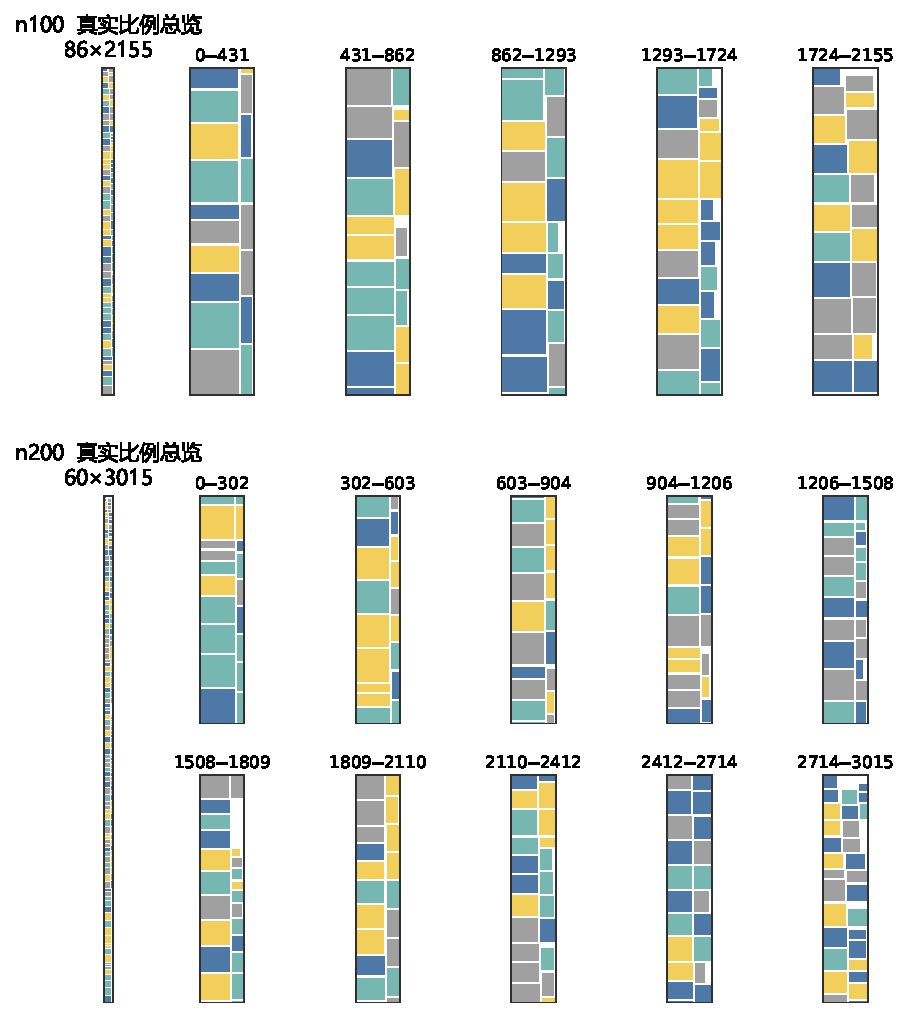
\includegraphics[width=\textwidth]{../results/q1/figures/q1_slender_overview_segments.pdf}
  \caption{\texttt{n100} 与 \texttt{n200} 的真实比例总览及分段展开。左列呈现完整外接轮廓，右侧依次展示连续纵向区段；低饱和颜色仅用于区分相邻模块。}
  \label{fig:q1_n100_n200}
\end{figure}

相对而言，\texttt{n300} 的 $520\times557$ 轮廓接近正方形，长短边比仅为 $1.0712$；与此同时，其面积冗余率上升至 $6.0292\%$。其真实比例布局见图~\ref{fig:q1_n300}。

\begin{figure}[H]
  \centering
  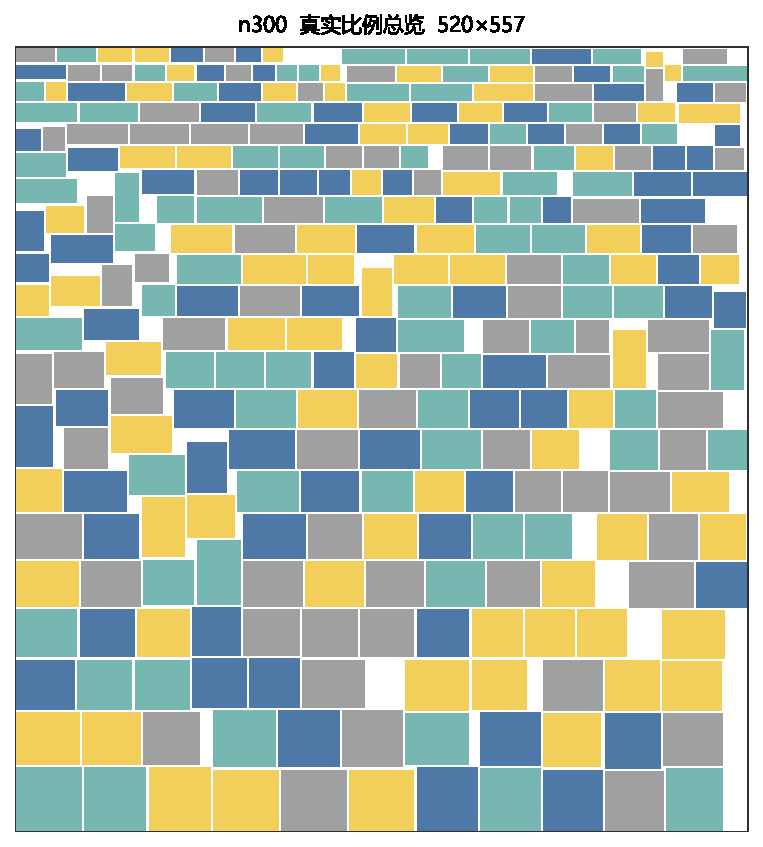
\includegraphics[width=0.78\textwidth]{../results/q1/figures/q1_n300_balanced_layout.pdf}
  \caption{\texttt{n300} 的真实比例布局。$520\times557$ 外接轮廓接近正方形，白色区域为模块间空隙。}
  \label{fig:q1_n300}
\end{figure}

综合三组实例，较低的面积冗余率并未保证接近正方形的外形，而更均衡的轮廓也可能伴随更高的面积冗余。由此可见，在本组自由轮廓算例中，\textbf{面积紧凑性与轮廓均衡性存在竞争关系}；词典序目标所规定的主次顺序，正是三组布局呈现不同形态的直接判优依据。

\subsection{模型结果检验}

最终坐标均通过模块完整性、两两非重叠和模块总面积一致性复核。Skyline 与 MaxRects 属于启发式构造，因此表~\ref{tab:q1_results}给出的是当前搜索范围内的可行上界，不能据此严格证明大规模实例的全局最优性。

至此，本问在保持面积优先判据的同时揭示了紧凑性与均衡性的竞争规律；所建立的模块旋转、非重叠约束与轮廓表示，也为后续加入固定边界、互连关系或形状扩展提供了基础。

\section{问题二：固定轮廓互连线长模型的建立与求解}

为了在给定死区率的正方形轮廓内降低模块互连线长，本问沿“网络驱动目标位置—几何合法化—局部线长优化”的技术主线展开：先由网络连接与固定 Terminal 提取模块的目标中心，再将这些连续目标转化为满足固定边界和非重叠约束的离散布局，最后修正合法化造成的局部线长损失。

\subsection{固定轮廓与 HPWL 优化模型}

\subsubsection{连续轮廓与整数坐标边界}

设硬模块总面积为 $A_{\mathrm{block}}$，题目给定死区率 $\Gamma=0.15$。按死区率定义，正方形轮廓面积及连续边长为
\begin{equation}
  A_{\mathrm{outline}}=(1+\Gamma)A_{\mathrm{block}},
  \qquad
  L_{\mathrm{box}}=\sqrt{(1+\Gamma)A_{\mathrm{block}}}.
  \label{eq:q2_outline}
\end{equation}
模块尺寸和模块坐标均为整数，因此模块右边界和上边界也是整数。令
\begin{equation}
  G=\lfloor L_{\mathrm{box}}\rfloor,
  \label{eq:q2_grid_side}
\end{equation}
则整数坐标下的 $x_i+w_i\le L_{\mathrm{box}}$ 与 $x_i+w_i\le G$ 等价，纵向边界同理。$G$ 仅用于确定整数坐标，轮廓面积仍由连续边长 $L_{\mathrm{box}}$ 按式~\eqref{eq:q2_outline}计算。由三组模块总面积得到的固定轮廓参数见表~\ref{tab:q2_outline_parameters}。

\begin{table}[H]
  \centering
  \caption{问题二固定正方形轮廓参数}
  \label{tab:q2_outline_parameters}
  \small
  \begin{tabular}{lrrrr}
    \toprule
    实例 & $A_{\mathrm{block}}$ & $L_{\mathrm{box}}$ & $G$ & $A_{\mathrm{outline}}$ \\
    \midrule
    \texttt{n100} & 179501 & 454.341 & 454 & 206426.150 \\
    \texttt{n200} & 175696 & 449.500 & 449 & 202050.400 \\
    \texttt{n300} & 273170 & 560.487 & 560 & 314145.500 \\
    \bottomrule
  \end{tabular}
\end{table}

由此先得到连续轮廓边长 $L_{\mathrm{box}}$，再由 $G$ 刻画与整数模块坐标等价的边界。问题二沿用问题一的旋转变量 $r_i$ 和旋转后尺寸 $(w_i,h_i)$；在固定正方形轮廓内，每个模块必须满足
\begin{equation}
  0\le x_i,\quad 0\le y_i,\quad
  x_i+w_i\le L_{\mathrm{box}},\quad y_i+h_i\le L_{\mathrm{box}}.
  \label{eq:q2_boundary}
\end{equation}
任意两个模块仍满足式~\eqref{eq:q1_nonoverlap}的方向分离约束。式~\eqref{eq:q2_boundary}与非重叠约束共同定义本问的几何可行域。

\subsubsection{模块中心、HPWL 与优化目标}

在上述整数坐标可行域中，模块引脚位于几何中心，因此模块 $i$ 的引脚坐标为
\begin{equation}
  \boldsymbol{c}_i=\left(x_i+\frac{w_i}{2},\ y_i+\frac{h_i}{2}\right).
  \label{eq:q2_block_center}
\end{equation}
若引脚 $p$ 属于硬模块，则 $(X_p,Y_p)=\boldsymbol{c}_i$；若其为外部终端，则 $(X_p,Y_p)$ 取 \texttt{.pl} 中的固定坐标。对网络 $e$，其半周长线长为
\begin{equation}
  \ell_e=
  \left(\max_{p\in\mathcal{P}_e}X_p-\min_{p\in\mathcal{P}_e}X_p\right)
  +
  \left(\max_{p\in\mathcal{P}_e}Y_p-\min_{p\in\mathcal{P}_e}Y_p\right).
  \label{eq:q2_net_hpwl}
\end{equation}
该指标等于网络所有引脚最小轴对齐外接矩形的半周长。全部网络的总 HPWL 为
\begin{equation}
  \mathcal{L}=\sum_{e\in\mathcal{E}}\ell_e.
  \label{eq:q2_total_hpwl}
\end{equation}

第二问要求在固定轮廓可行域内最小化式~\eqref{eq:q2_total_hpwl}，可写为
\begin{equation}
  \begin{aligned}
    \min_{\{x_i,y_i,r_i\}}\quad & \mathcal{L},\\
    \text{s.t.}\quad
      & r_i\in\{0,1\},\quad x_i,y_i\in\mathbb{Z}_{\ge0},\\
      & \text{式~\eqref{eq:q1_rotation}、\eqref{eq:q1_nonoverlap}和~\eqref{eq:q2_boundary}}.
  \end{aligned}
  \label{eq:q2_model}
\end{equation}
至此，连续边长 $L_{\mathrm{box}}$ 决定物理轮廓，整数边界 $G$ 决定坐标可行域，模块中心将几何位置映射为网络引脚位置，单网 HPWL 再汇总为总 HPWL，最终形成式~\eqref{eq:q2_model}的优化目标。由于旋转、坐标和模块相对位置均为离散决策，且非重叠条件为析取约束，下面采用分层方法在网络方向与几何可行性之间建立联系。

\subsection{求解方法：网络驱动合法化与局部重插入}

\subsubsection{二次线长松弛}

为获得模块在网络连接意义下的空间方向，暂时忽略非重叠约束，并以二次线长近似代替分段线性的 HPWL~\cite{eisenmann1998}。对引脚数为 $d_e$ 的网络，将其引脚两两连接成团，权重取 $1/(d_e-1)$，求解
\begin{equation}
  \min_{\{\boldsymbol{z}_i\}}
  \sum_{e\in\mathcal{E}}\frac{1}{d_e-1}
  \sum_{\substack{u<v\\u,v\in\mathcal{P}_e}}
  \lVert\boldsymbol{z}_u-\boldsymbol{z}_v\rVert_2^2,
  \label{eq:q2_quadratic_relaxation}
\end{equation}
其中外部 Terminal 位置保持固定，硬模块中心为待求变量。式~\eqref{eq:q2_quadratic_relaxation}形成图拉普拉斯线性方程，求解后将模块中心投影到轮廓坐标范围，得到目标中心 $\widehat{\boldsymbol{c}}_i$。必须强调，该松弛解只用于提供网络驱动的空间方向：它既未满足模块非重叠等离散几何约束，也不是最终 HPWL 解。

\subsubsection{目标引导几何合法化}

二次松弛得到的目标中心通常彼此重叠，不能直接作为模块坐标。合法化虽然能够消除越界与重叠，却会迫使模块偏离其网络目标位置；而逐个放置的先后关系还会改变剩余空间形态，使早期几何决策被后续模块继承。因此，合法化并非单纯的可行性修补，它可能破坏松弛解中已经形成的网络邻近结构，并成为最终 HPWL 的重要来源。

为降低这种损失，本文在固定轮廓的可用矩形区域内逐个插入模块，使候选位置同时参考目标中心、已放置相邻引脚与固定 Terminal 所提供的局部网络信息，并在两种旋转方向下检验边界和重叠约束。考虑到模块顺序会形成不同的空间分割结构，再以网络连接、模块几何特征和目标中心位置构造多种初始顺序，并以不同侧重点的插入准则扩充可行初值。最终统一按精确总 HPWL 比较这些合法布局。

\subsubsection{局部重插入：合法化损失的二次修正}

几何合法化首先保证可行，但未必使每个模块处于对其关联网络最有利的位置。为对这部分线长损失进行二次修正，本文按模块的 HPWL 贡献依次尝试单模块重插入：\texttt{n100} 在移除模块后重新确定可用矩形区域，\texttt{n200} 和 \texttt{n300} 则利用相邻引脚、Terminal 与目标中心形成的 HPWL 断点控制搜索规模。每次调整均重新检验几何约束，且只有精确总 HPWL 严格下降时才接受，从而在不破坏合法性的前提下恢复部分网络邻近关系。当前实现仅对初始 HPWL 较小的若干布局进行有限轮局部修正；具体预算为前 $3$ 个布局和 $2$ 轮迭代。

第二问的求解步骤如下：
\begin{enumerate}
  \item 读取模块、网络和终端数据，计算 $A_{\mathrm{block}}$、$L_{\mathrm{box}}$ 与 $G$；
  \item 求解二次线长松弛，得到模块目标中心；
  \item 组合多种初始顺序和插入准则，在 $G\times G$ 整数坐标区域内得到可行布局；
  \item 对较优初始布局进行局部重插入，修正合法化造成的线长损失；
  \item 根据最终模块坐标重新计算 HPWL，并选择其中最小的可行布局；
  \item 检验模块完整性、边界、重叠、面积与 HPWL 一致性，得到模块坐标和布局图。
\end{enumerate}

解析松弛需要求解规模为模块数的线性方程组，稠密实现的计算复杂度为 $O(n^3)$；合法化与局部重插入还需反复检验候选区域和模块冲突，因此大规模实例采用 HPWL 断点搜索控制计算量。

\subsection{求解结果与分析}

\subsubsection{HPWL 求解结果}

表~\ref{tab:q2_main_results}给出各实例经过局部优化后的 HPWL 最小可行布局。局部改善率以对应合法化初始布局的 HPWL 为基准计算。

\begin{table}[H]
  \centering
  \caption{问题二固定轮廓下的 HPWL 优化结果}
  \label{tab:q2_main_results}
  \small
  \resizebox{\textwidth}{!}{%
  \begin{tabular}{lrrrrrl}
    \toprule
    实例 & $L_{\mathrm{box}}$ & 初始 HPWL & 最终 HPWL & 改善率/\% & 有效移动次数 & 局部改进方法 \\
    \midrule
    \texttt{n100} & 454.341 & 224273.0 & 220279.0 & 1.7809 & 44 & 精确空矩形重插入 \\
    \texttt{n200} & 449.500 & 411599.0 & 410072.5 & 0.3709 & 20 & HPWL 断点搜索 \\
    \texttt{n300} & 560.487 & 563981.0 & 560492.5 & 0.6185 & 34 & HPWL 断点搜索 \\
    \bottomrule
  \end{tabular}%
  }
\end{table}

三组数据经过局部重插入后 HPWL 均继续下降：\texttt{n100} 由 $224273.0$ 降至 $220279.0$，改善 $1.7809\%$；\texttt{n200} 与 \texttt{n300} 分别改善 $0.3709\%$ 和 $0.6185\%$。这说明几何合法化虽然已经给出可行布局，但模块相对位置中仍保留可被局部移动利用的线长优化空间，也验证了“合法化后再修正”这一层次的必要性。为直观比较三组数据的变化，将表中优化前后的 HPWL 绘于图~\ref{fig:q2_hpwl_before_after}。

\begin{figure}[H]
  \centering
  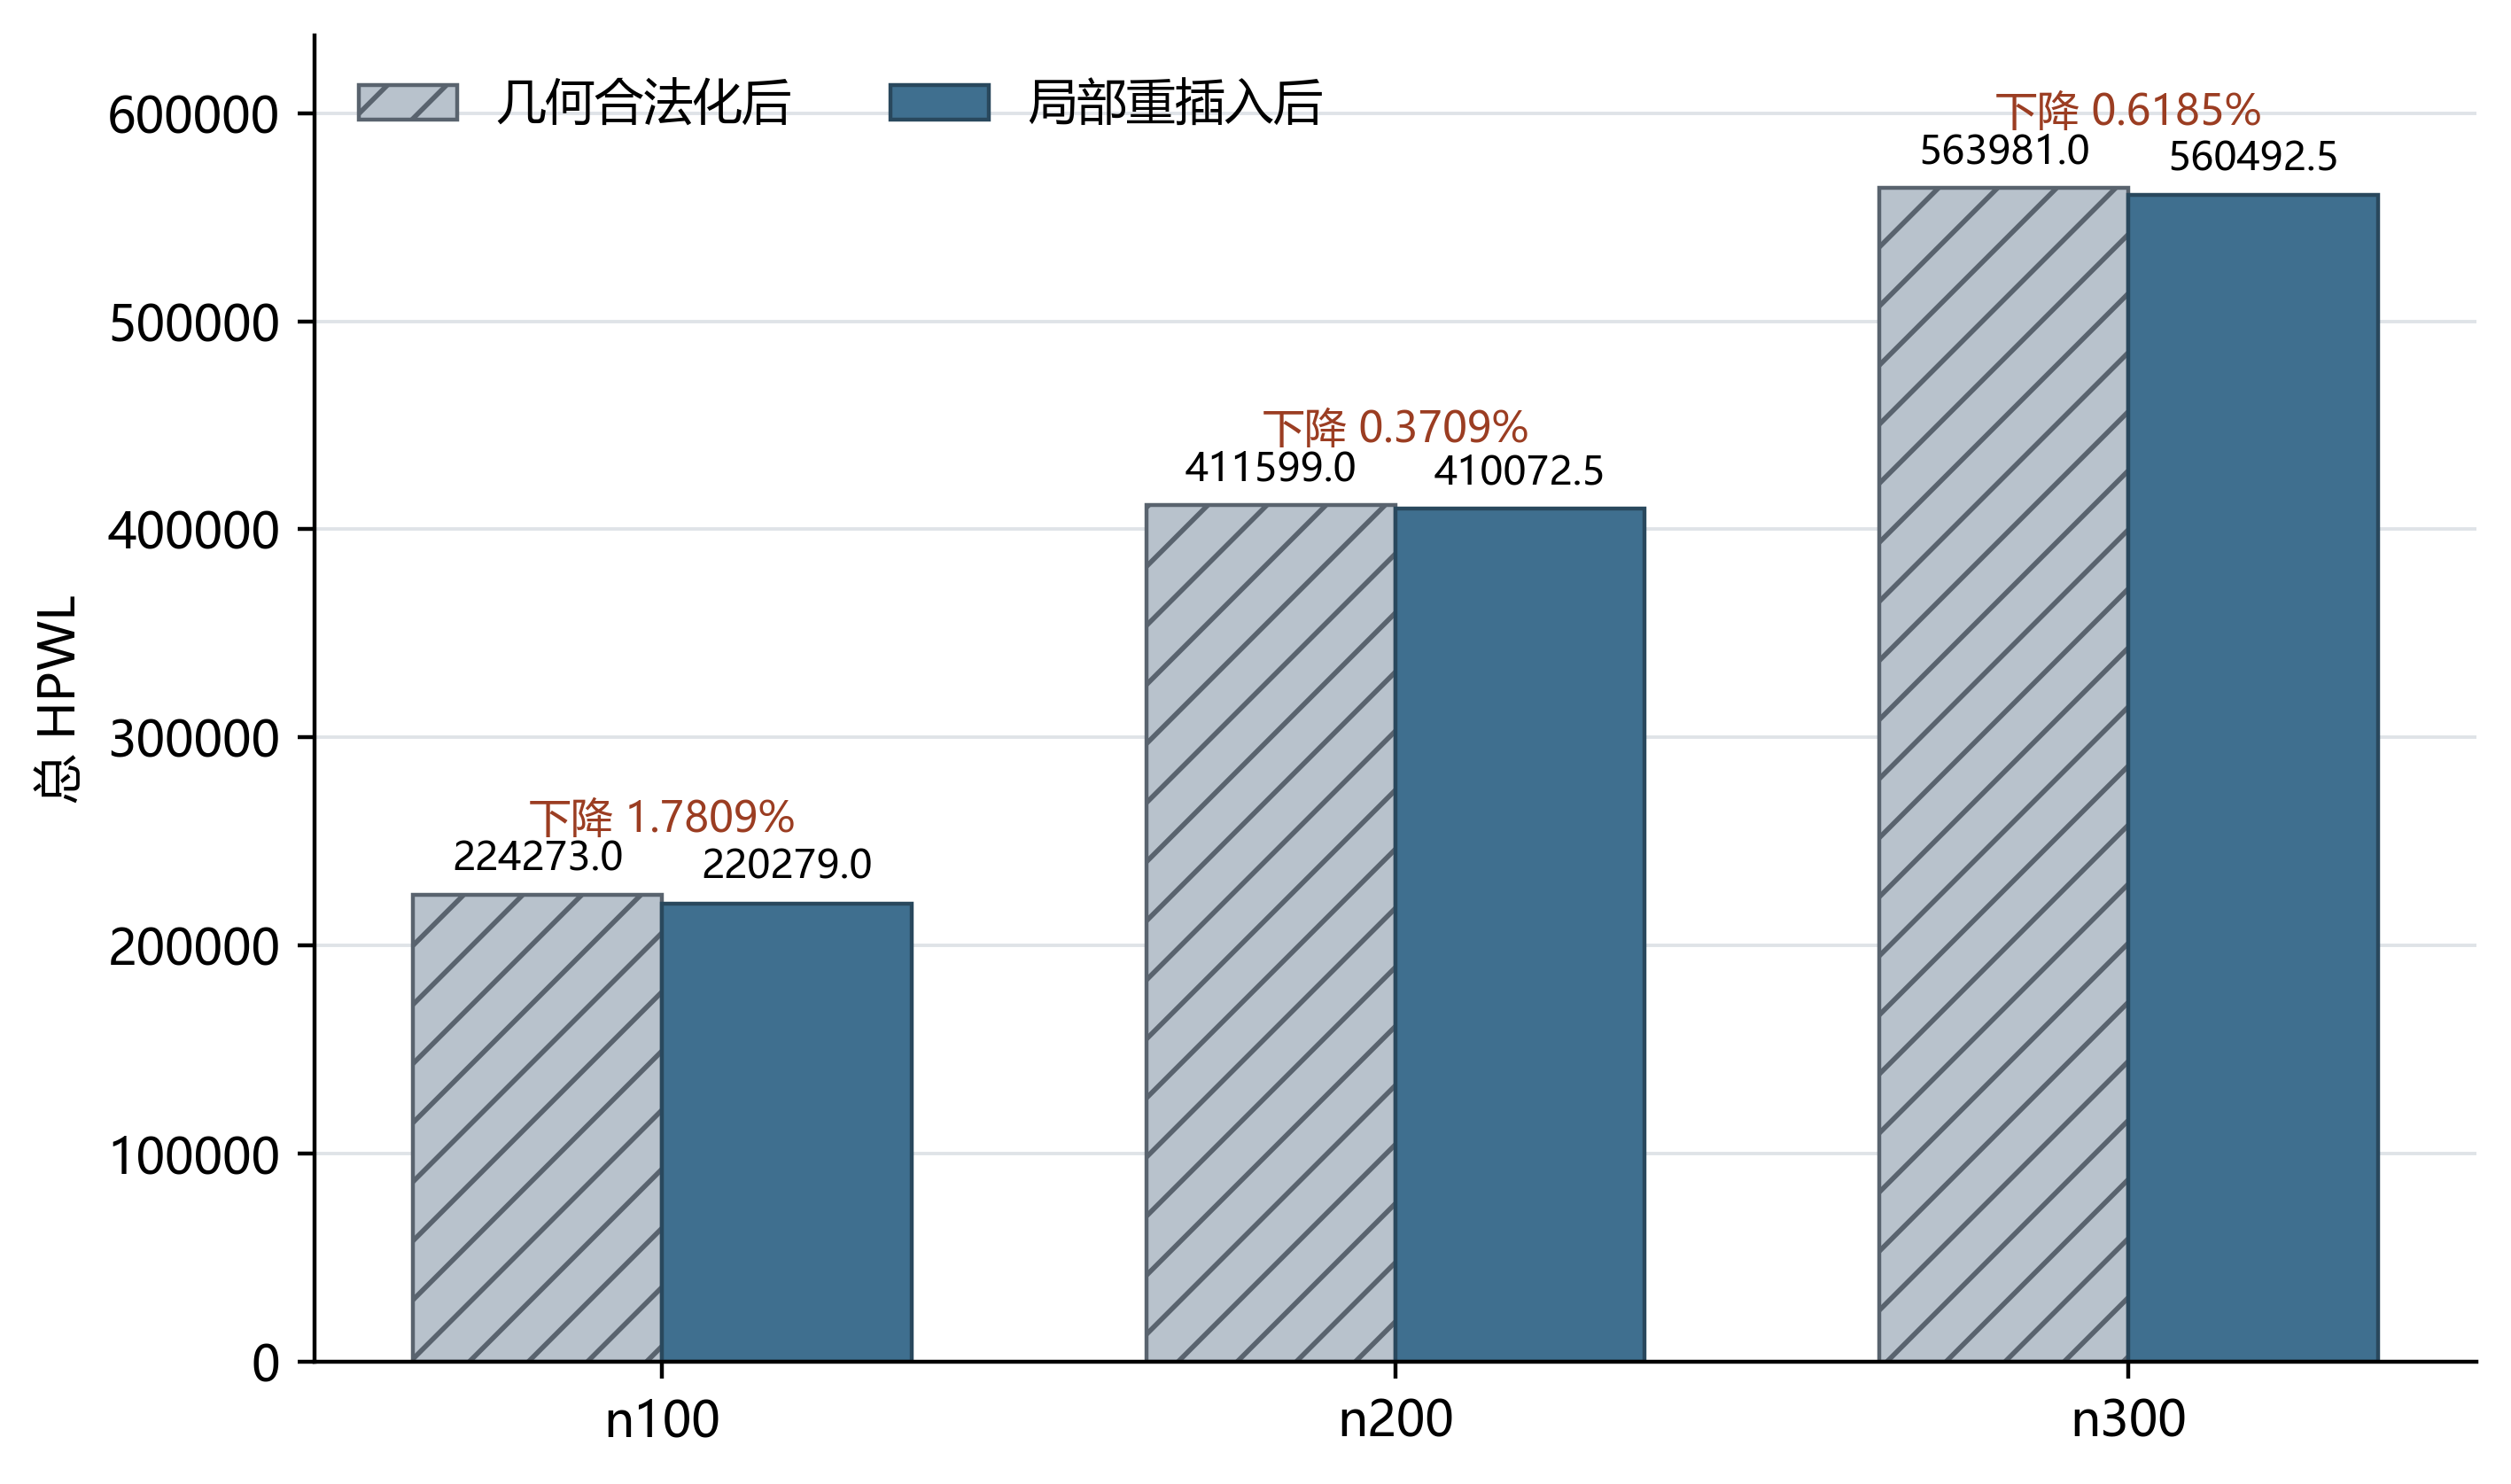
\includegraphics[width=0.78\textwidth]{../results/q2/figures/q2_hpwl_before_after.png}
  \caption{三组实例在几何合法化后与局部重插入后的 HPWL 对比}
  \label{fig:q2_hpwl_before_after}
\end{figure}

图中三组柱对均呈下降关系，其中 \texttt{n100} 的相对降幅最大；\texttt{n200} 和 \texttt{n300} 的降幅较小但方向一致。局部优化的作用因而不是重新构造布局，而是在固定轮廓和既有空间分割结构下，进一步回收合法化造成的局部线长损失。

\subsubsection{初始布局依赖性分析}

表~\ref{tab:q2_candidate_comparison}并非一般的方法优劣对照，而用于考察初始合法化结构对最终结果的影响。每组实例列出三个代表性合法布局及其局部优化结果，表内 HPWL 均由对应布局坐标按同一公式重新计算。

\begin{table}[H]
  \centering
  \caption{问题二局部搜索结果对初始合法化布局的依赖性}
  \label{tab:q2_candidate_comparison}
  \small
  \begin{tabular}{l p{4.4cm} rrr}
    \toprule
    实例 & 方法组合 & 初始 HPWL & 改进后 HPWL & 有效移动次数 \\
    \midrule
    \texttt{n100} & \texttt{degree\_area+wire} & 224273.0 & 220279.0 & 44 \\
    \texttt{n100} & \texttt{shelf\_bfd:native} & 242944.0 & 233349.0 & 109 \\
    \texttt{n100} & \texttt{area\_degree+target} & 243190.5 & 234380.5 & 32 \\
    \midrule
    \texttt{n200} & \texttt{target\_yx+wire} & 411599.0 & 410072.5 & 20 \\
    \texttt{n200} & \texttt{degree\_area+wire} & 413258.0 & 412640.5 & 27 \\
    \texttt{n200} & \texttt{area\_degree+wire} & 420230.5 & 417335.0 & 47 \\
    \midrule
    \texttt{n300} & \texttt{target\_xy+wire} & 563981.0 & 560492.5 & 34 \\
    \texttt{n300} & \texttt{target\_yx+wire} & 582961.5 & 576107.0 & 59 \\
    \texttt{n300} & \texttt{degree\_area+wire} & 600456.5 & 593534.5 & 47 \\
    \bottomrule
  \end{tabular}
\end{table}

表中所有代表性布局经过局部搜索后 HPWL 均下降，说明局部修正具有一致作用；但同一实例的改进后 HPWL 仍存在明显差异。其原因在于，不同初始顺序和插入准则会在合法化阶段形成不同的模块邻接关系与剩余空间分割，而单模块局部搜索只能在既有结构附近调整，难以跨越较大的结构性差异。因此，局部搜索不能完全消除初始合法化的影响，构造多初值并从中筛选具有必要性。这也表明，最终 HPWL 不仅取决于局部移动能力，更取决于网络驱动信息在合法化阶段被保留的程度。

为展示固定轮廓内的模块分布及线长压力，将 \texttt{n100} 和 \texttt{n200} 的布局并列绘于图~\ref{fig:q2_n100_n200}。图中低饱和色矩形表示普通硬模块，黑点表示固定 Terminal，统一强调色矩形表示 HPWL 较高网络的引脚外接框。

\begin{figure}[H]
  \centering
  \begin{minipage}[c]{0.48\textwidth}
    \centering
    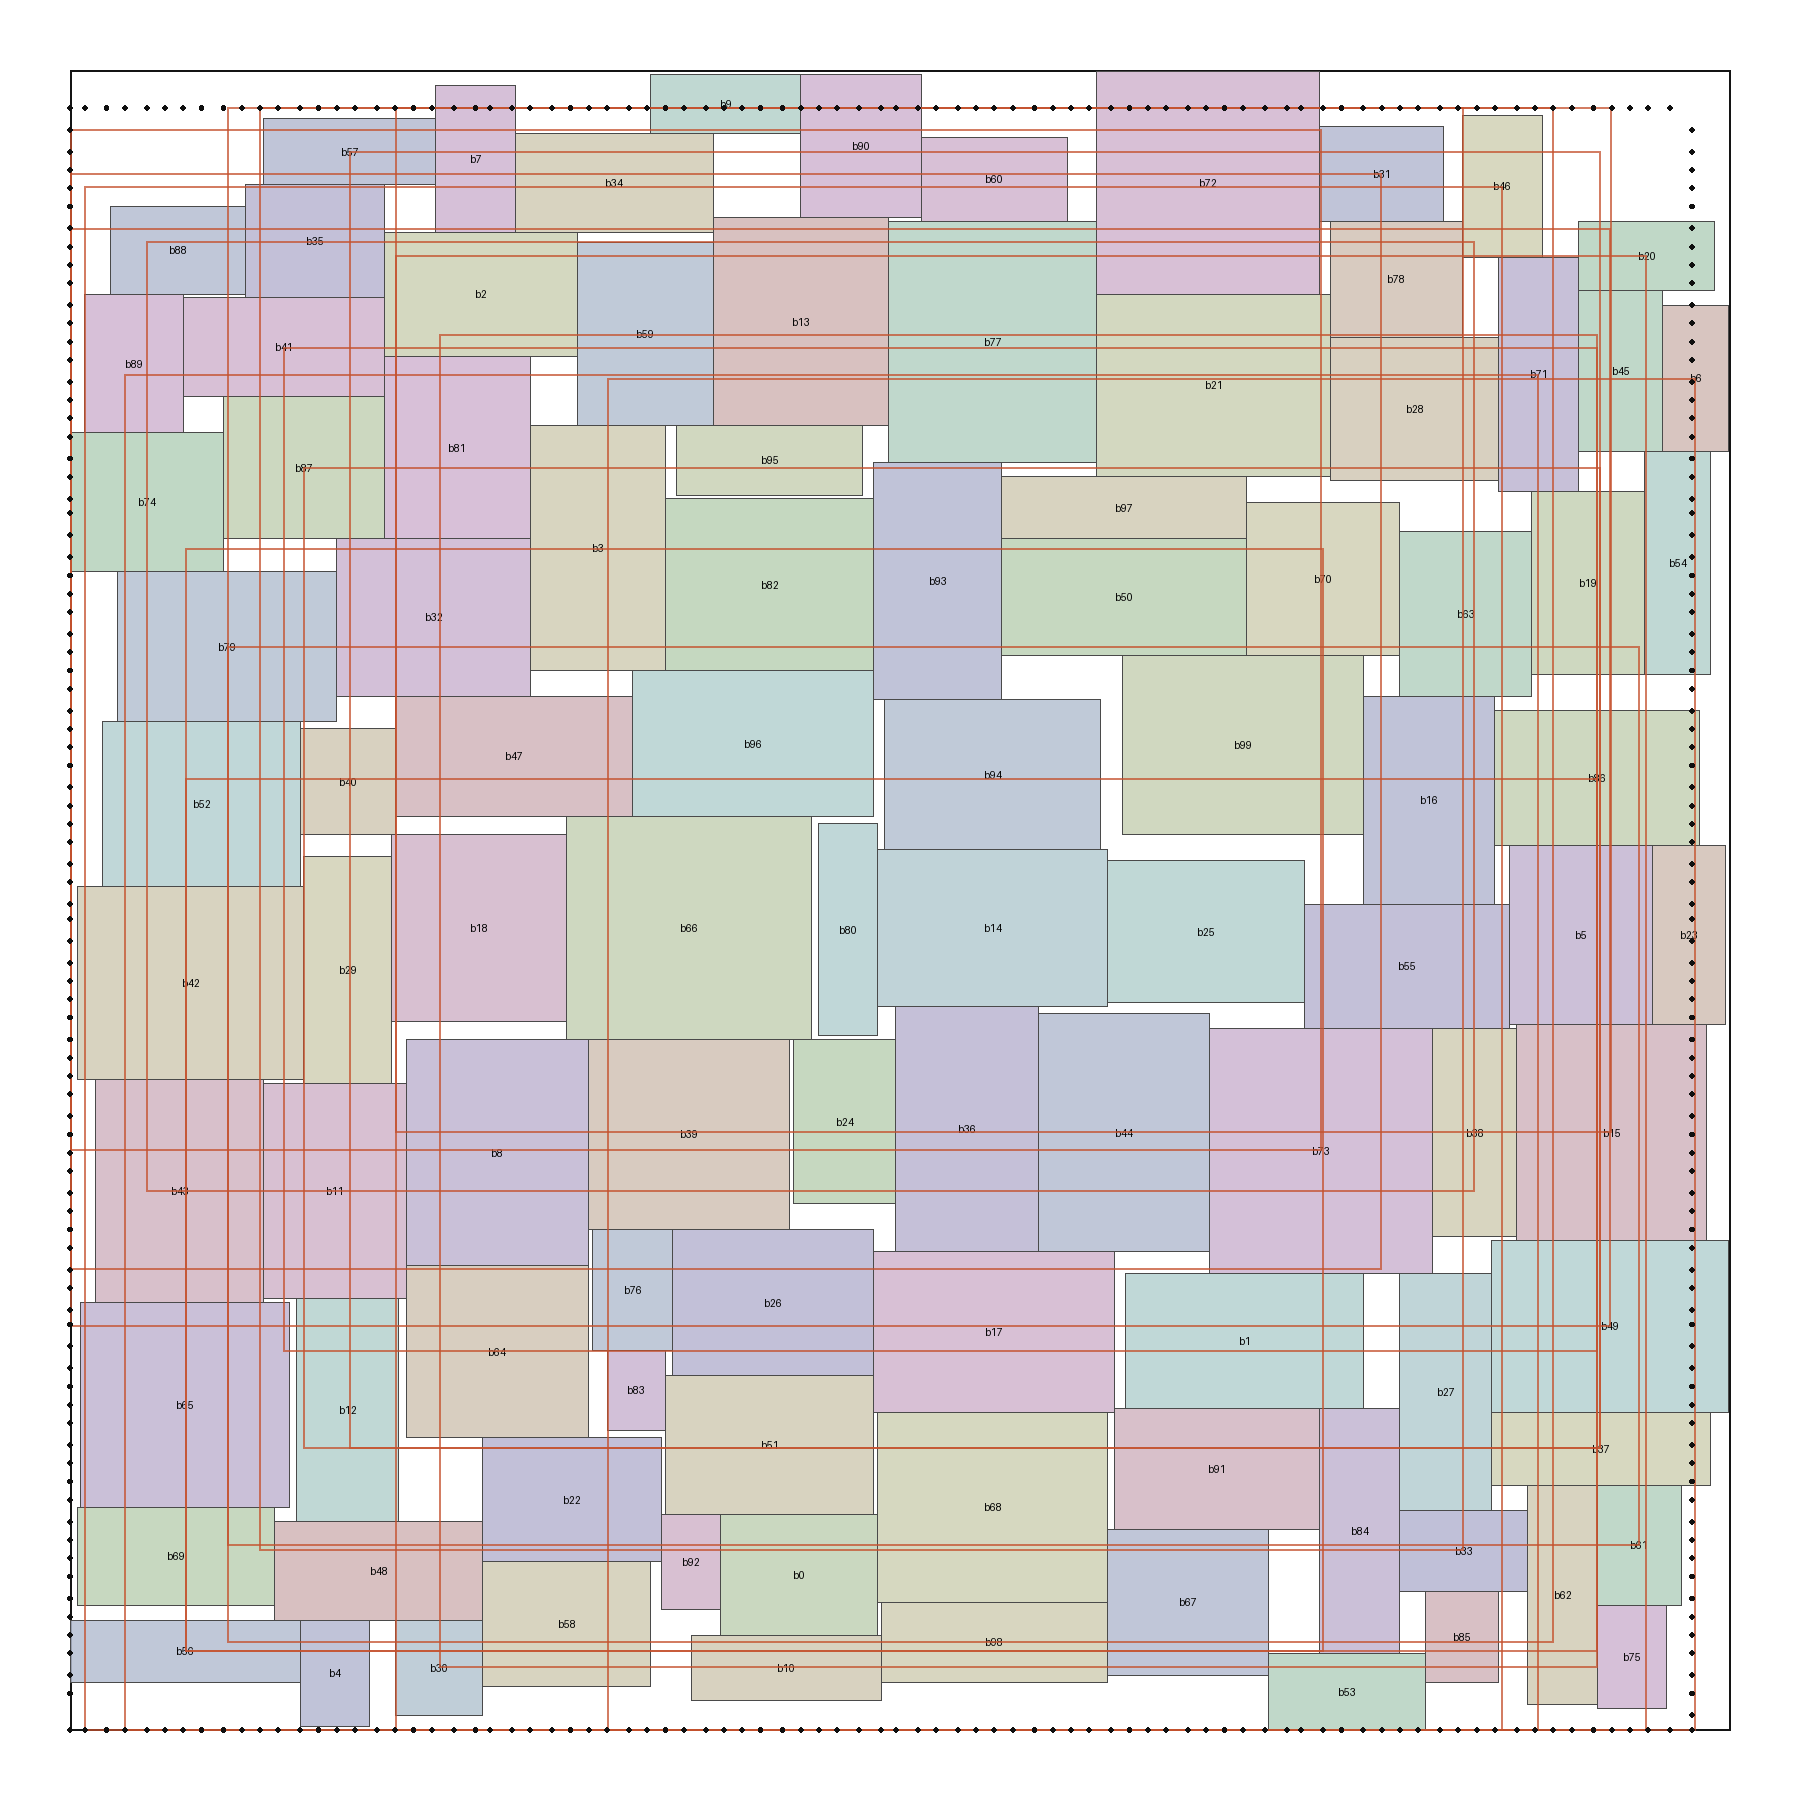
\includegraphics[width=\textwidth]{../results/q2/figures/n100_q2_layout.png}\\[-0.3em]
    {\small (a) \texttt{n100}}
  \end{minipage}
  \hfill
  \begin{minipage}[c]{0.48\textwidth}
    \centering
    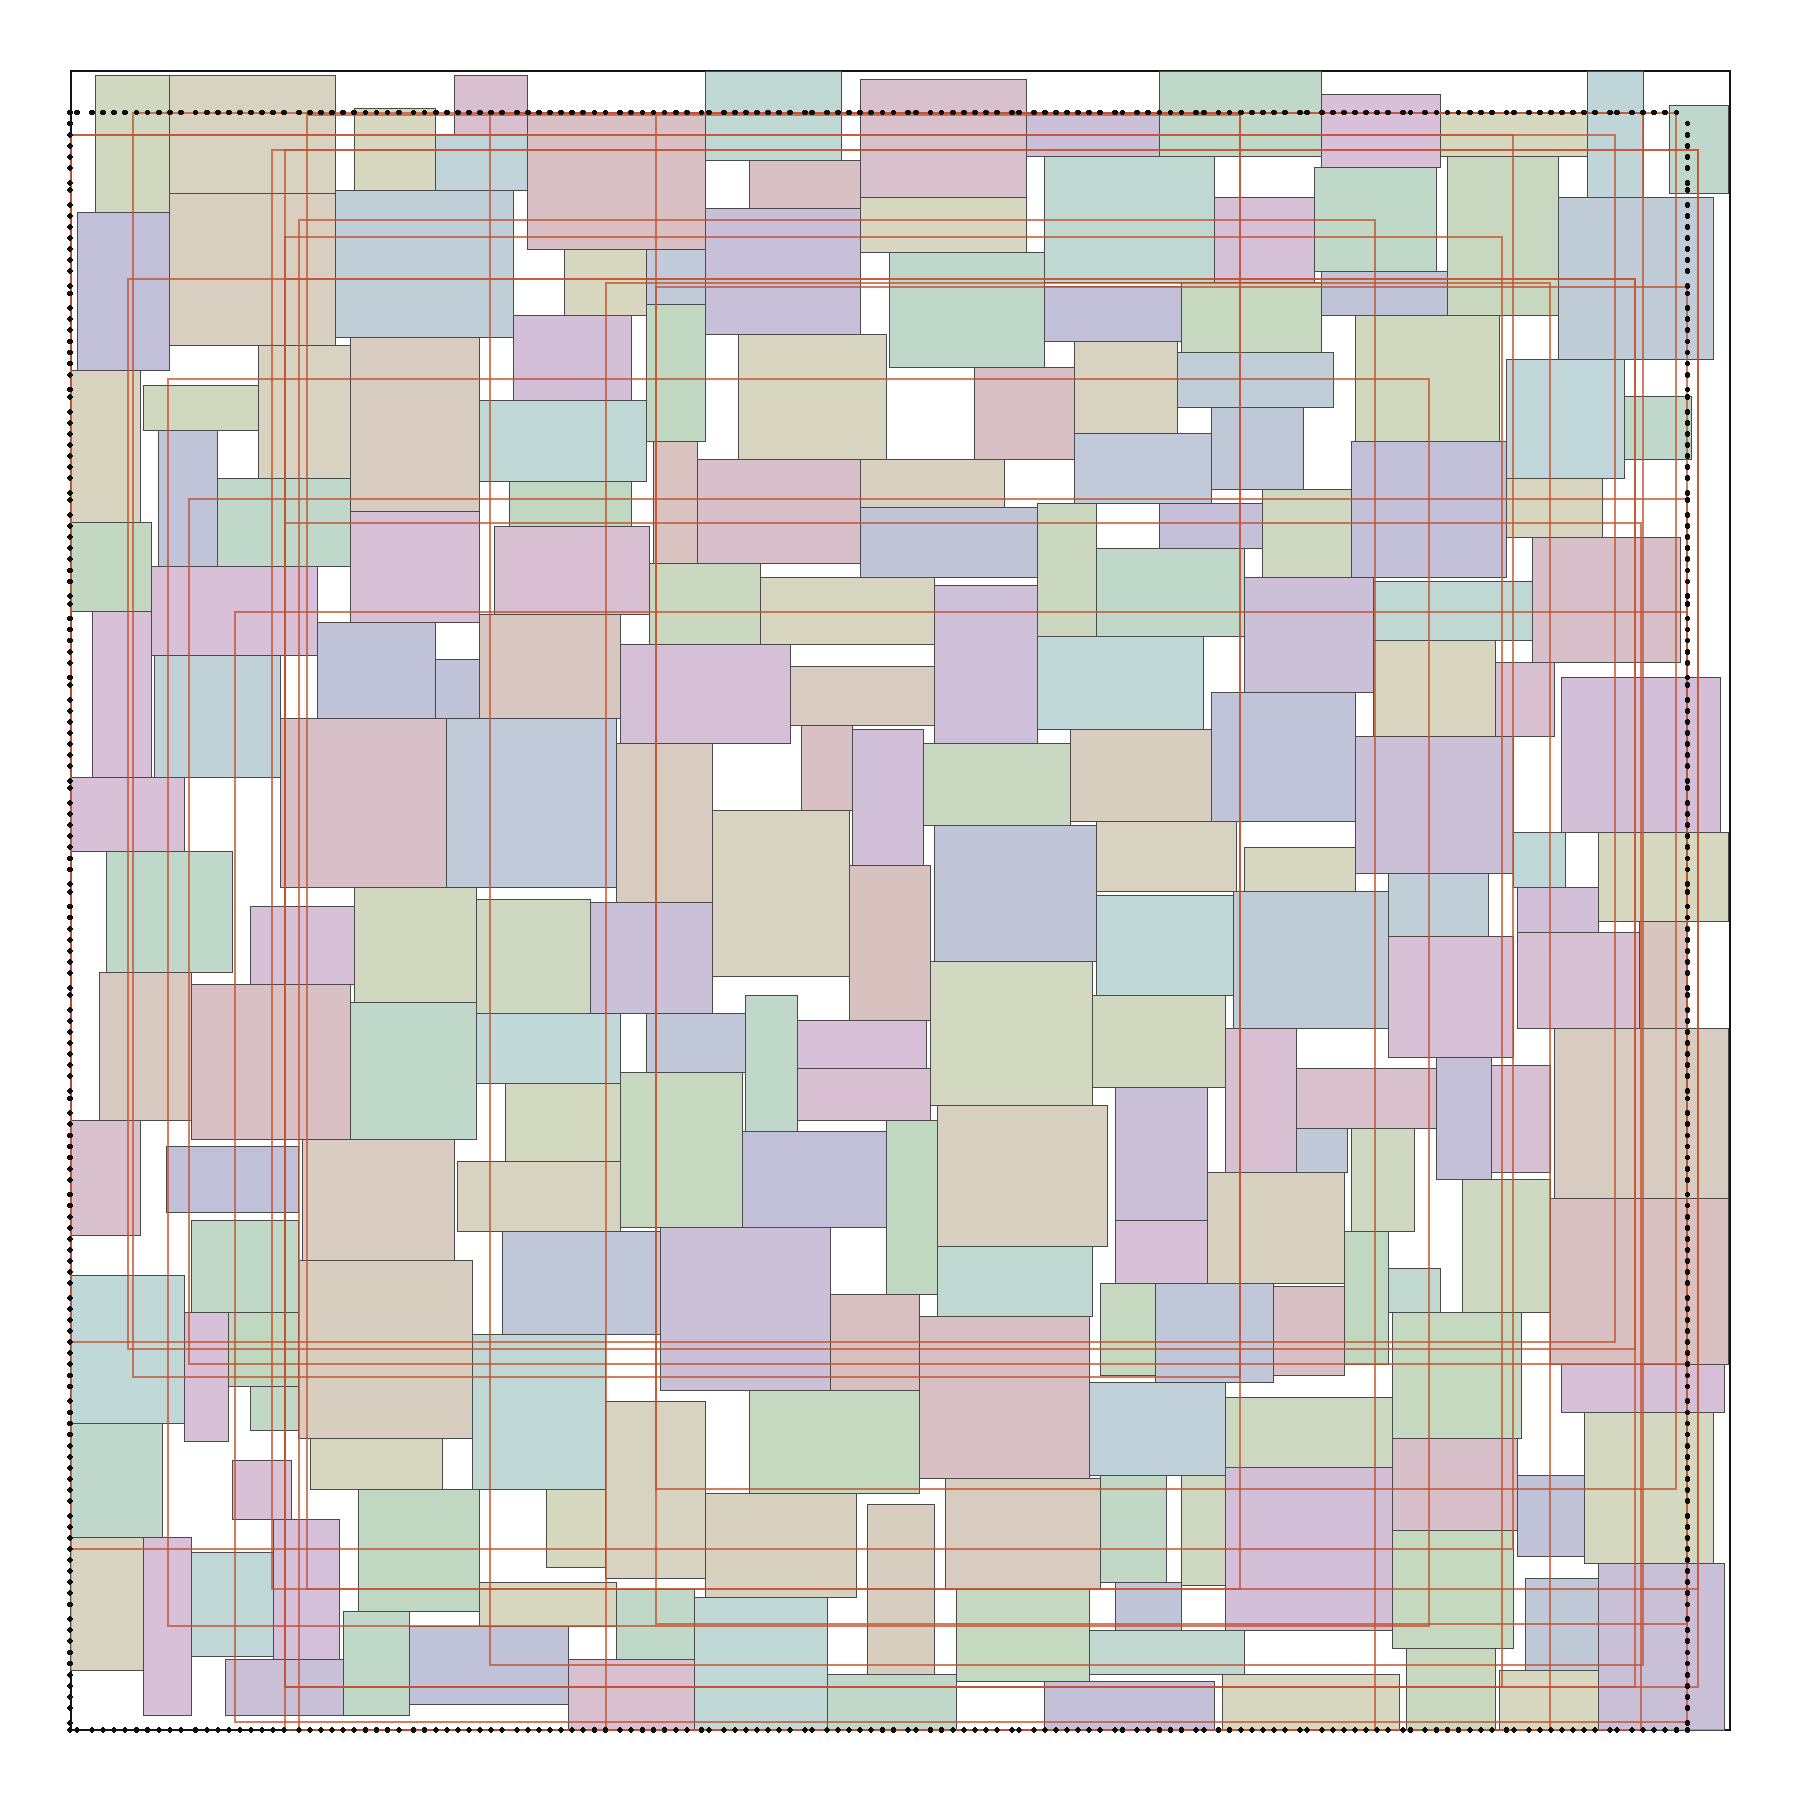
\includegraphics[width=\textwidth]{../results/q2/figures/n200_q2_layout.png}\\[-0.3em]
    {\small (b) \texttt{n200}}
  \end{minipage}
  \caption{问题二 \texttt{n100} 与 \texttt{n200} 在死区率 $0.15$ 下的固定轮廓 HPWL 布局。外黑框为连续正方形轮廓。}
  \label{fig:q2_n100_n200}
\end{figure}

两组布局均将全部模块限制在正方形边界内，同时保留由式~\eqref{eq:q2_outline}规定的空余空间。强调色网络外接框跨越多个模块区域，反映出固定 Terminal 和多引脚网络对模块相对位置的共同约束；普通模块采用低饱和配色，使视觉注意力集中于这些线长压力较高的网络。

\texttt{n300} 包含 $300$ 个硬模块和 $1893$ 条网络，其最终布局见图~\ref{fig:q2_n300}。

\begin{figure}[H]
  \centering
  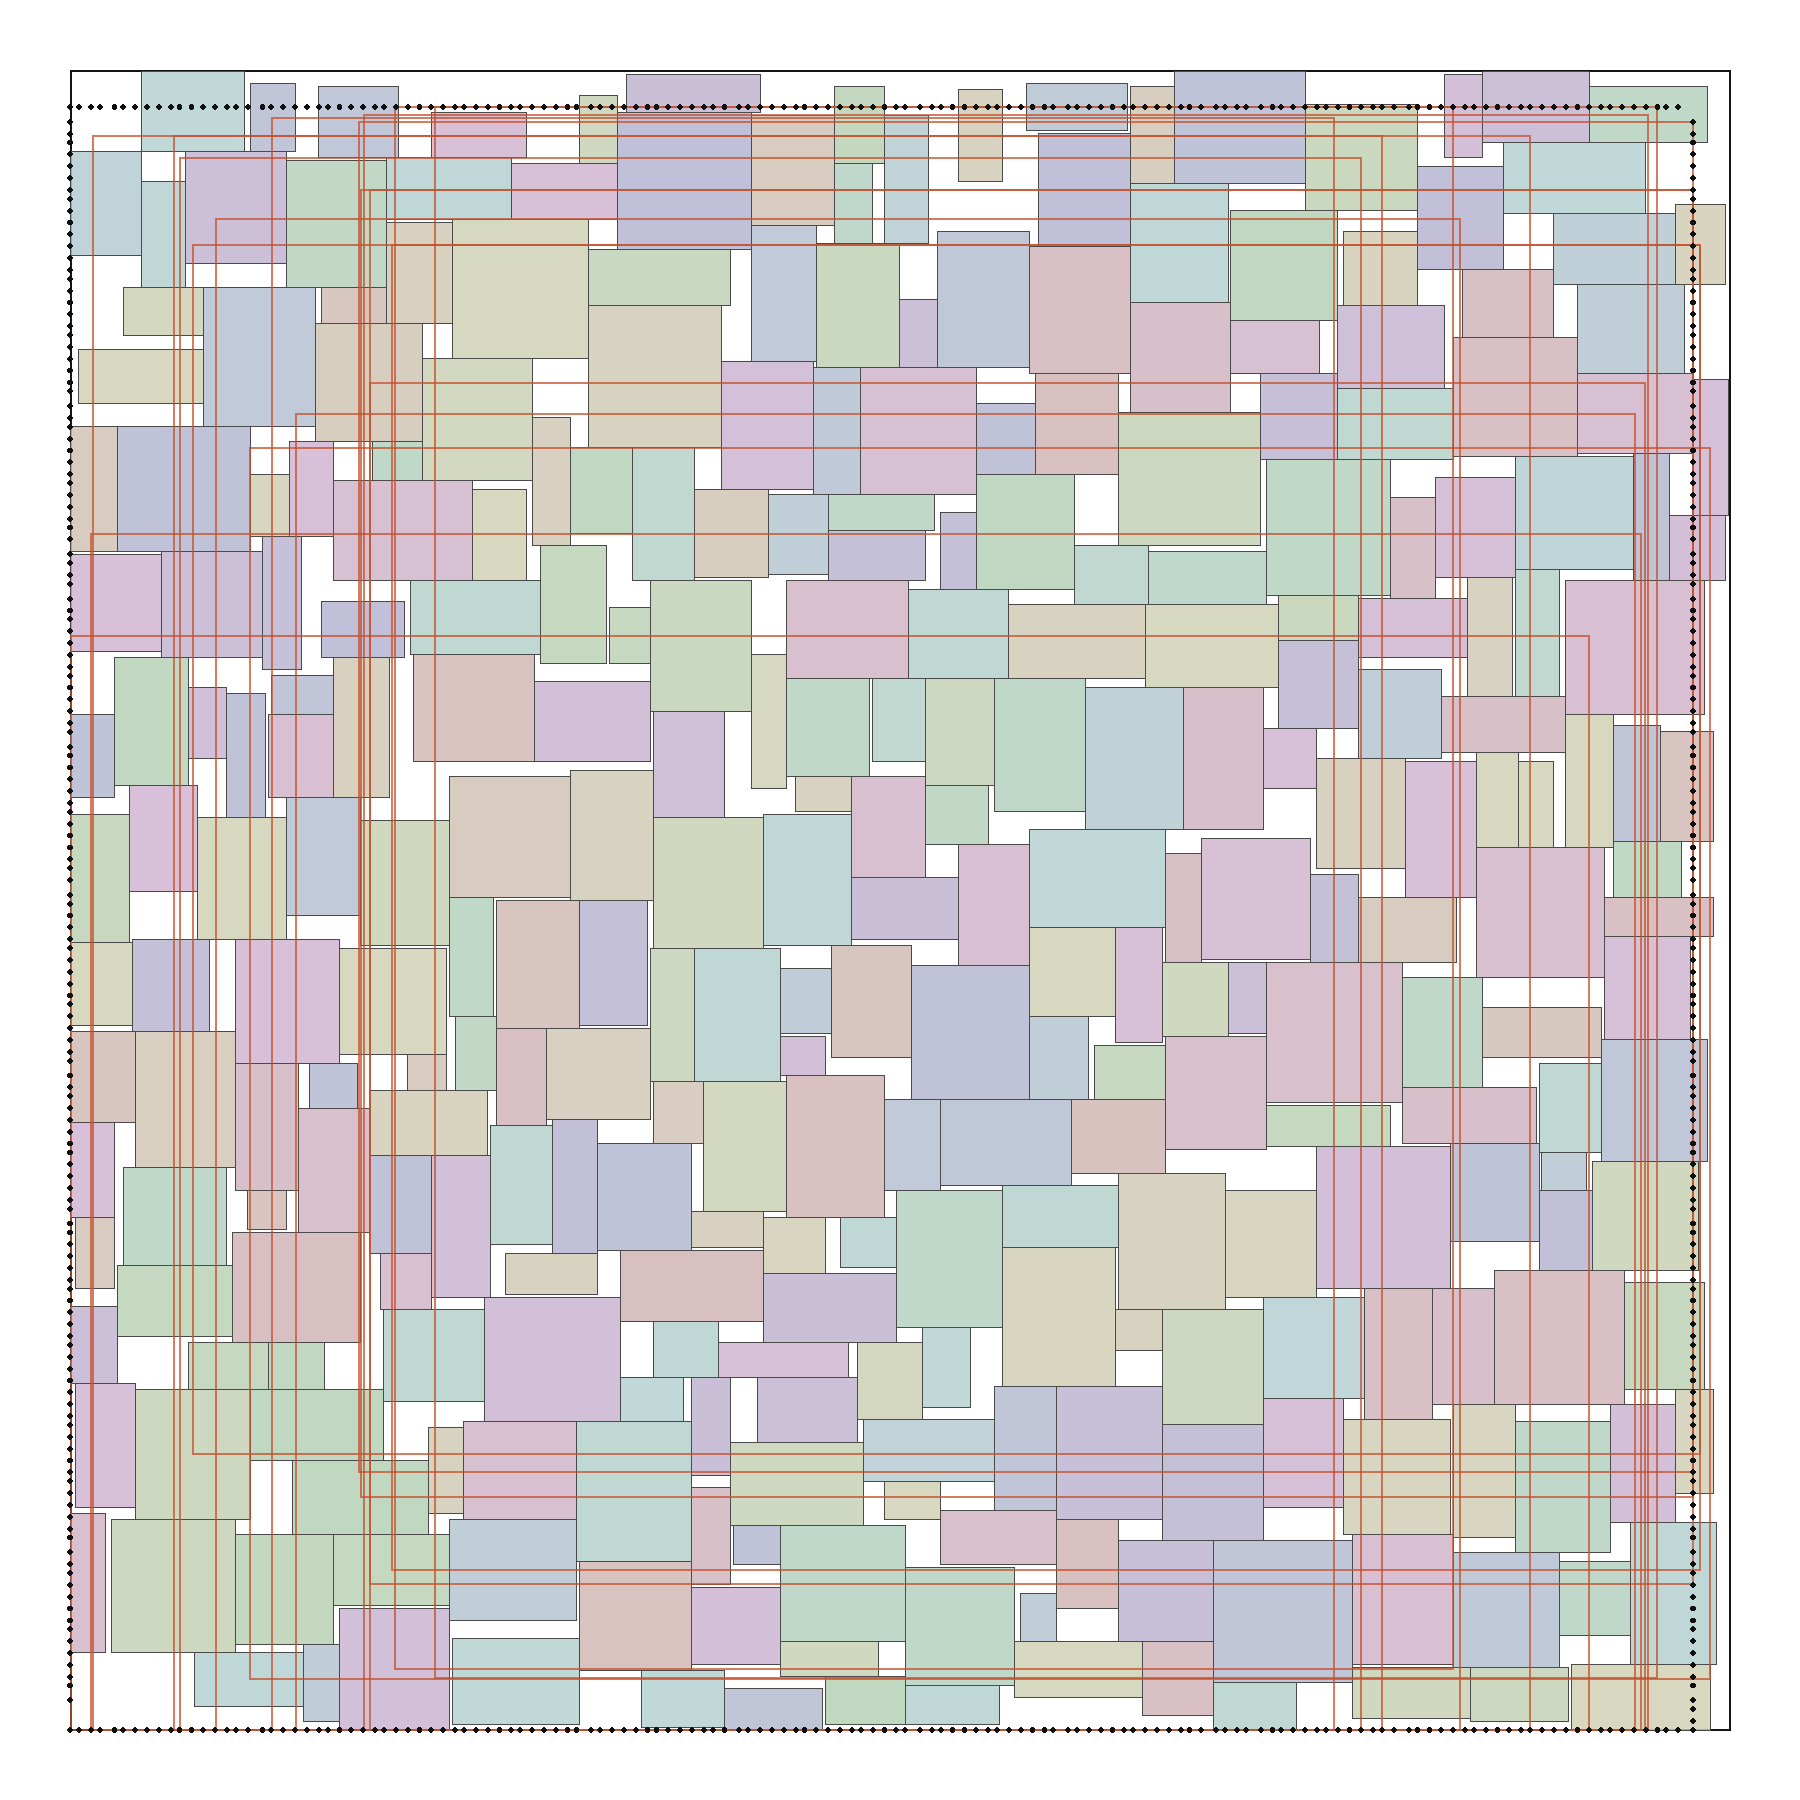
\includegraphics[width=0.88\textwidth]{../results/q2/figures/n300_q2_layout.png}
  \caption{问题二 \texttt{n300} 在连续边长 $560.487$ 的正方形轮廓内所得 HPWL 布局。白色区域为未被硬模块占用的空间。}
  \label{fig:q2_n300}
\end{figure}

在模块和网络规模增加后，布局仍满足相同的固定轮廓与死区率定义。其最终半周长线长为 $560492.5$，相较局部优化前降低 $3488.5$，说明断点局部搜索在保持几何可行性的同时进一步缩短了网络外接框半周长之和。固定轮廓矩形布局含有大规模析取约束，二次松弛、合法化和局部重插入均属于启发式求解，因此上述 HPWL 是经验证的可行结果，不构成全局最优性证明。

\subsection{模型结果检验}

三组最终布局均通过模块完整性、连续轮廓边界、两两非重叠、模块总面积一致性与 HPWL 独立复算检验；详细复核结果移至附录表~\ref{tab:appendix_q2_validation}。

问题二在死区率 $0.15$ 的固定正方形轮廓内完成三组硬模块布局，所得总\allowbreak HPWL 分别为\allowbreak $220279.0$、$410072.5$ 和 $560492.5$。结果表明，网络驱动目标中心为几何布局提供了方向，但初始合法化保留网络结构的程度仍会影响局部搜索后的最终 HPWL；本问方法可进一步用于问题三不同死区率下的布局求解。

\section{问题三：轮廓压缩与线长优化模型的建立与求解}

问题三将问题二的固定死区率推广为正方形整数边长搜索。本文先利用面积与模块尺寸确定轮廓下界，再按边长逐一构造布局，并在当前搜索策略首次成功构造全部模块的边长下复用问题二的网络驱动优化，由此考察死区率下降所带来的 HPWL 代价。

\subsection{轮廓压缩的词典序模型}

\subsubsection{面积下界、模块下界与搜索边长}

设全部硬模块的总面积为
\begin{equation}
  A_{\mathrm{block}}=\sum_i w_i^0h_i^0.
  \label{eq:q3_block_area}
\end{equation}
若正方形轮廓边长为整数 $S$，则面积必要条件和单模块尺寸必要条件分别给出
\begin{equation}
  S_{\mathrm{area}}=\left\lceil\sqrt{A_{\mathrm{block}}}\right\rceil,
  \qquad
  S_{\mathrm{block}}=\max_i\max(w_i^0,h_i^0),
  \label{eq:q3_lower_bounds}
\end{equation}
从而搜索下界为
\begin{equation}
  S_{\mathrm{lb}}=\max\left(S_{\mathrm{area}},S_{\mathrm{block}}\right).
  \label{eq:q3_search_lb}
\end{equation}
三组实例的下界分解以及问题二提供的已知可行边长上界见表~\ref{tab:q3_search_bounds}。

\begin{table}[H]
  \centering
  \caption{问题三整数轮廓边长的搜索区间}
  \label{tab:q3_search_bounds}
  \small
  \renewcommand{\arraystretch}{1.15}
  \begin{tabular}{c r r r r r}
    \toprule
    实例 & $A_{\mathrm{block}}$ & $S_{\mathrm{area}}$ & $S_{\mathrm{block}}$ & $S_{\mathrm{lb}}$ & 问题二整数上界 \\
    \midrule
    \texttt{n100} & 179501 & 424 & 67 & 424 & 454 \\
    \texttt{n200} & 175696 & 420 & 48 & 420 & 449 \\
    \texttt{n300} & 273170 & 523 & 48 & 523 & 560 \\
    \bottomrule
  \end{tabular}
\end{table}

对于任一候选边长 $S\ge S_{\mathrm{lb}}$，旋转后的模块宽高仍由式~(\ref{eq:q1_rotation}) 确定，并满足
\begin{equation}
  0\le x_i,\quad 0\le y_i,\quad
  x_i+w_i\le S,\quad y_i+h_i\le S,
  \label{eq:q3_boundary}
\end{equation}
以及式~(\ref{eq:q1_nonoverlap}) 的两两非重叠约束。

\subsubsection{死区率与词典序目标}

候选边长 $S$ 对应的死区率为
\begin{equation}
  \Gamma(S)=\frac{S^2-A_{\mathrm{block}}}{A_{\mathrm{block}}}.
  \label{eq:q3_deadspace}
\end{equation}
由于 $A_{\mathrm{block}}$ 固定，$\Gamma(S)$ 随 $S$ 严格单调增加，故最小化死区率等价于最小化 $S$。题目优化顺序是先压缩轮廓、再控制线长，因此以式~(\ref{eq:q2_total_hpwl}) 定义的总 HPWL $\mathcal{L}$ 为第二层目标，建立
\begin{equation}
  \operatorname{lexmin}\left(S,\mathcal{L}\right),
  \quad
  \text{s.t. 式~(\ref{eq:q3_boundary}) 和式~(\ref{eq:q1_nonoverlap})成立}.
  \label{eq:q3_lex_model}
\end{equation}
这一目标保持了题目给定的优先级，也避免为面积与线长人为设置权重。

本文将轮廓解释为硬模块的摆放边界：固定 Terminal 仅作为网络引脚参与 HPWL，不计入硬模块面积，也不受该边界约束。该解释下，问题三的主模型依次由 $A_{\mathrm{block}}$、$S_{\mathrm{area}}$ 与 $S_{\mathrm{block}}$、$S_{\mathrm{lb}}$、候选 $S$、$\Gamma(S)$ 和 $\operatorname{lexmin}(S,\mathcal{L})$ 构成；替代题意口径在第 9 节进行敏感性分析，相应诊断计数列于附录 A.2。

\subsection{整数边长搜索与网络驱动优化}

\subsubsection{从理论下界逐整数搜索轮廓}

对每组实例，从 $S_{\mathrm{lb}}$ 到问题二的整数合法化边界逐一枚举 $S$。在每个边长下，组合 MaxRects 的最短边适配、面积适配和最长边适配规则，以及面积、长边、短边和长宽比四种模块排序方式，并允许模块旋转；仅当全部模块均被放入 $S\times S$ 轮廓时，才记录该边长并终止外层搜索。

MaxRects 不是装箱可行性的完备判定器：小于 $S_{\mathrm{found}}$ 的边长未成功构造布局，只说明当前启发式策略搜索失败，不能证明数学不可行。因此，$S_{\mathrm{found}}$ 统一称为“当前搜索策略获得的最小成功构造边长”。

\subsubsection{成功构造边长下复用问题二的线长优化}

固定 $S=S_{\mathrm{found}}$ 后，继续采用问题二的 HPWL 优化方法：先由二次线长松弛求得模块目标中心，再通过行带构造和目标引导合法化生成确定性初始布局，按初始 HPWL 选取前 $3$ 个候选进行两轮单模块局部重插入。其中，\texttt{n100} 使用精确空矩形重插入，\texttt{n200} 与 \texttt{n300} 使用 HPWL 断点搜索，最终按复算后的 HPWL 选择布局。该过程保持整数边长搜索、MaxRects 策略和问题二线长优化方法不变。

\subsection{死区率---HPWL 权衡结果与机制分析}

三组实例的轮廓压缩与线长结果见表~\ref{tab:q3_main_results}。当前搜索策略获得的最小成功构造边长分别为 $439$、$432$、$537$；相较问题二统一设定的 $15\%$ 死区率，问题三将死区率压缩至 $7.3649\%$、$6.2198\%$、$5.5639\%$。与此同时，总 HPWL 分别由 $220279.0$、$410072.5$、$560492.5$ 增至 $239551.0$、$442024.0$、$640695.5$，相对增加约 $8.75\%$、$7.79\%$、$14.31\%$。

\begin{table}[H]
  \centering
  \caption{问题三轮廓压缩与 HPWL 权衡结果}
  \label{tab:q3_main_results}
  \small
  \renewcommand{\arraystretch}{1.15}
  \begin{tabular}{c r r r r r r}
    \toprule
    实例 & $S_{\mathrm{lb}}$ & $S_{\mathrm{found}}$ & 死区率/\% & 问题二 HPWL & 问题三 HPWL & 增量/\% \\
    \midrule
    \texttt{n100} & 424 & 439 & 7.3649 & 220279.0 & 239551.0 & 8.7489 \\
    \texttt{n200} & 420 & 432 & 6.2198 & 410072.5 & 442024.0 & 7.7917 \\
    \texttt{n300} & 523 & 537 & 5.5639 & 560492.5 & 640695.5 & 14.3094 \\
    \bottomrule
  \end{tabular}
\end{table}

为使面积利用率改善与互连代价处于同一视觉主线上，图~\ref{fig:q3_tradeoff} 分别绘制问题二到问题三的死区率变化和以问题二为基准的 HPWL 指数变化。

\begin{figure}[H]
  \centering
  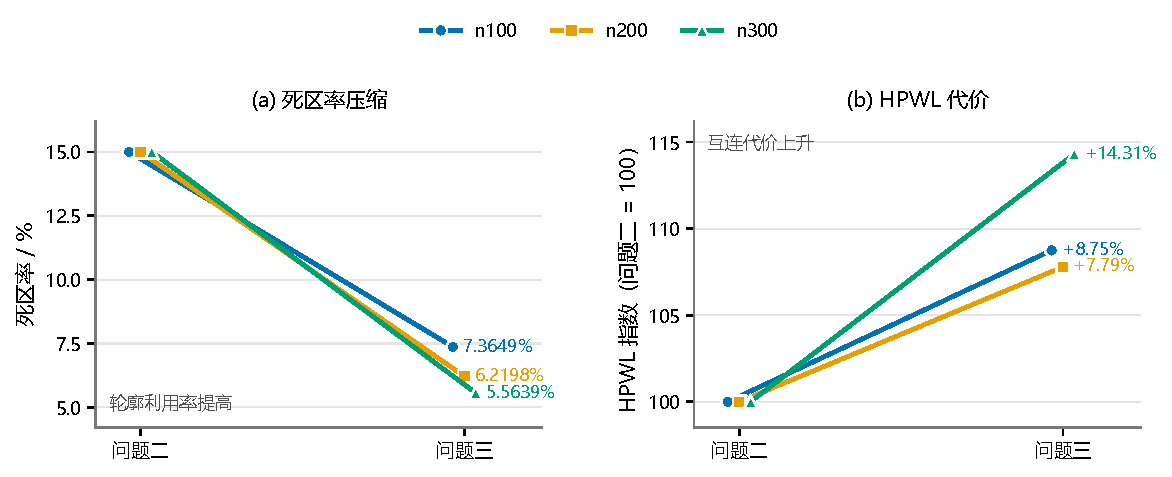
\includegraphics[width=0.88\textwidth]{../results/q3/figures/q3_tradeoff_q2_q3.pdf}
  \caption{问题二到问题三的死区率压缩与 HPWL 增长关系}
  \label{fig:q3_tradeoff}
\end{figure}

图~\ref{fig:q3_tradeoff} 左侧三条线均明显下降，而右侧三条线同时上升，直接呈现“更低死区率---更高互连线长”的权衡。轮廓压缩减少了可供模块平移、旋转和重插入的空隙，也限制了模块围绕网络目标中心调整的空间；因此，几何利用率提高的代价是互连结构受到更强的空间约束，网络外接框难以同时收缩，最终表现为总 HPWL 上升。这一变化是词典序目标先满足轮廓压缩所产生的结果，而非单一线长优化阶段的失效。

在三组实例中，\texttt{n300} 的 HPWL 增幅最大。结果表明其对空间压缩更敏感；结合该实例更大的模块与网络规模，这一现象提示：当更多模块和网络共同竞争有限的调整空间时，紧轮廓可能更快削弱线长优化的自由度，但该观察仅限于当前三组算例。

固定最小成功构造边长后，两轮局部搜索分别保留 $89$、$81$、$69$ 次有效移动，并将 HPWL 从 $244183.0$、$442742.5$、$644858.0$ 降至表~\ref{tab:q3_main_results} 所列结果，说明紧轮廓内仍有局部改善空间。对应布局见图~\ref{fig:q3_n100_n200} 和图~\ref{fig:q3_n300}。

\begin{figure}[H]
  \centering
  \begin{minipage}[t]{0.48\textwidth}
    \centering
    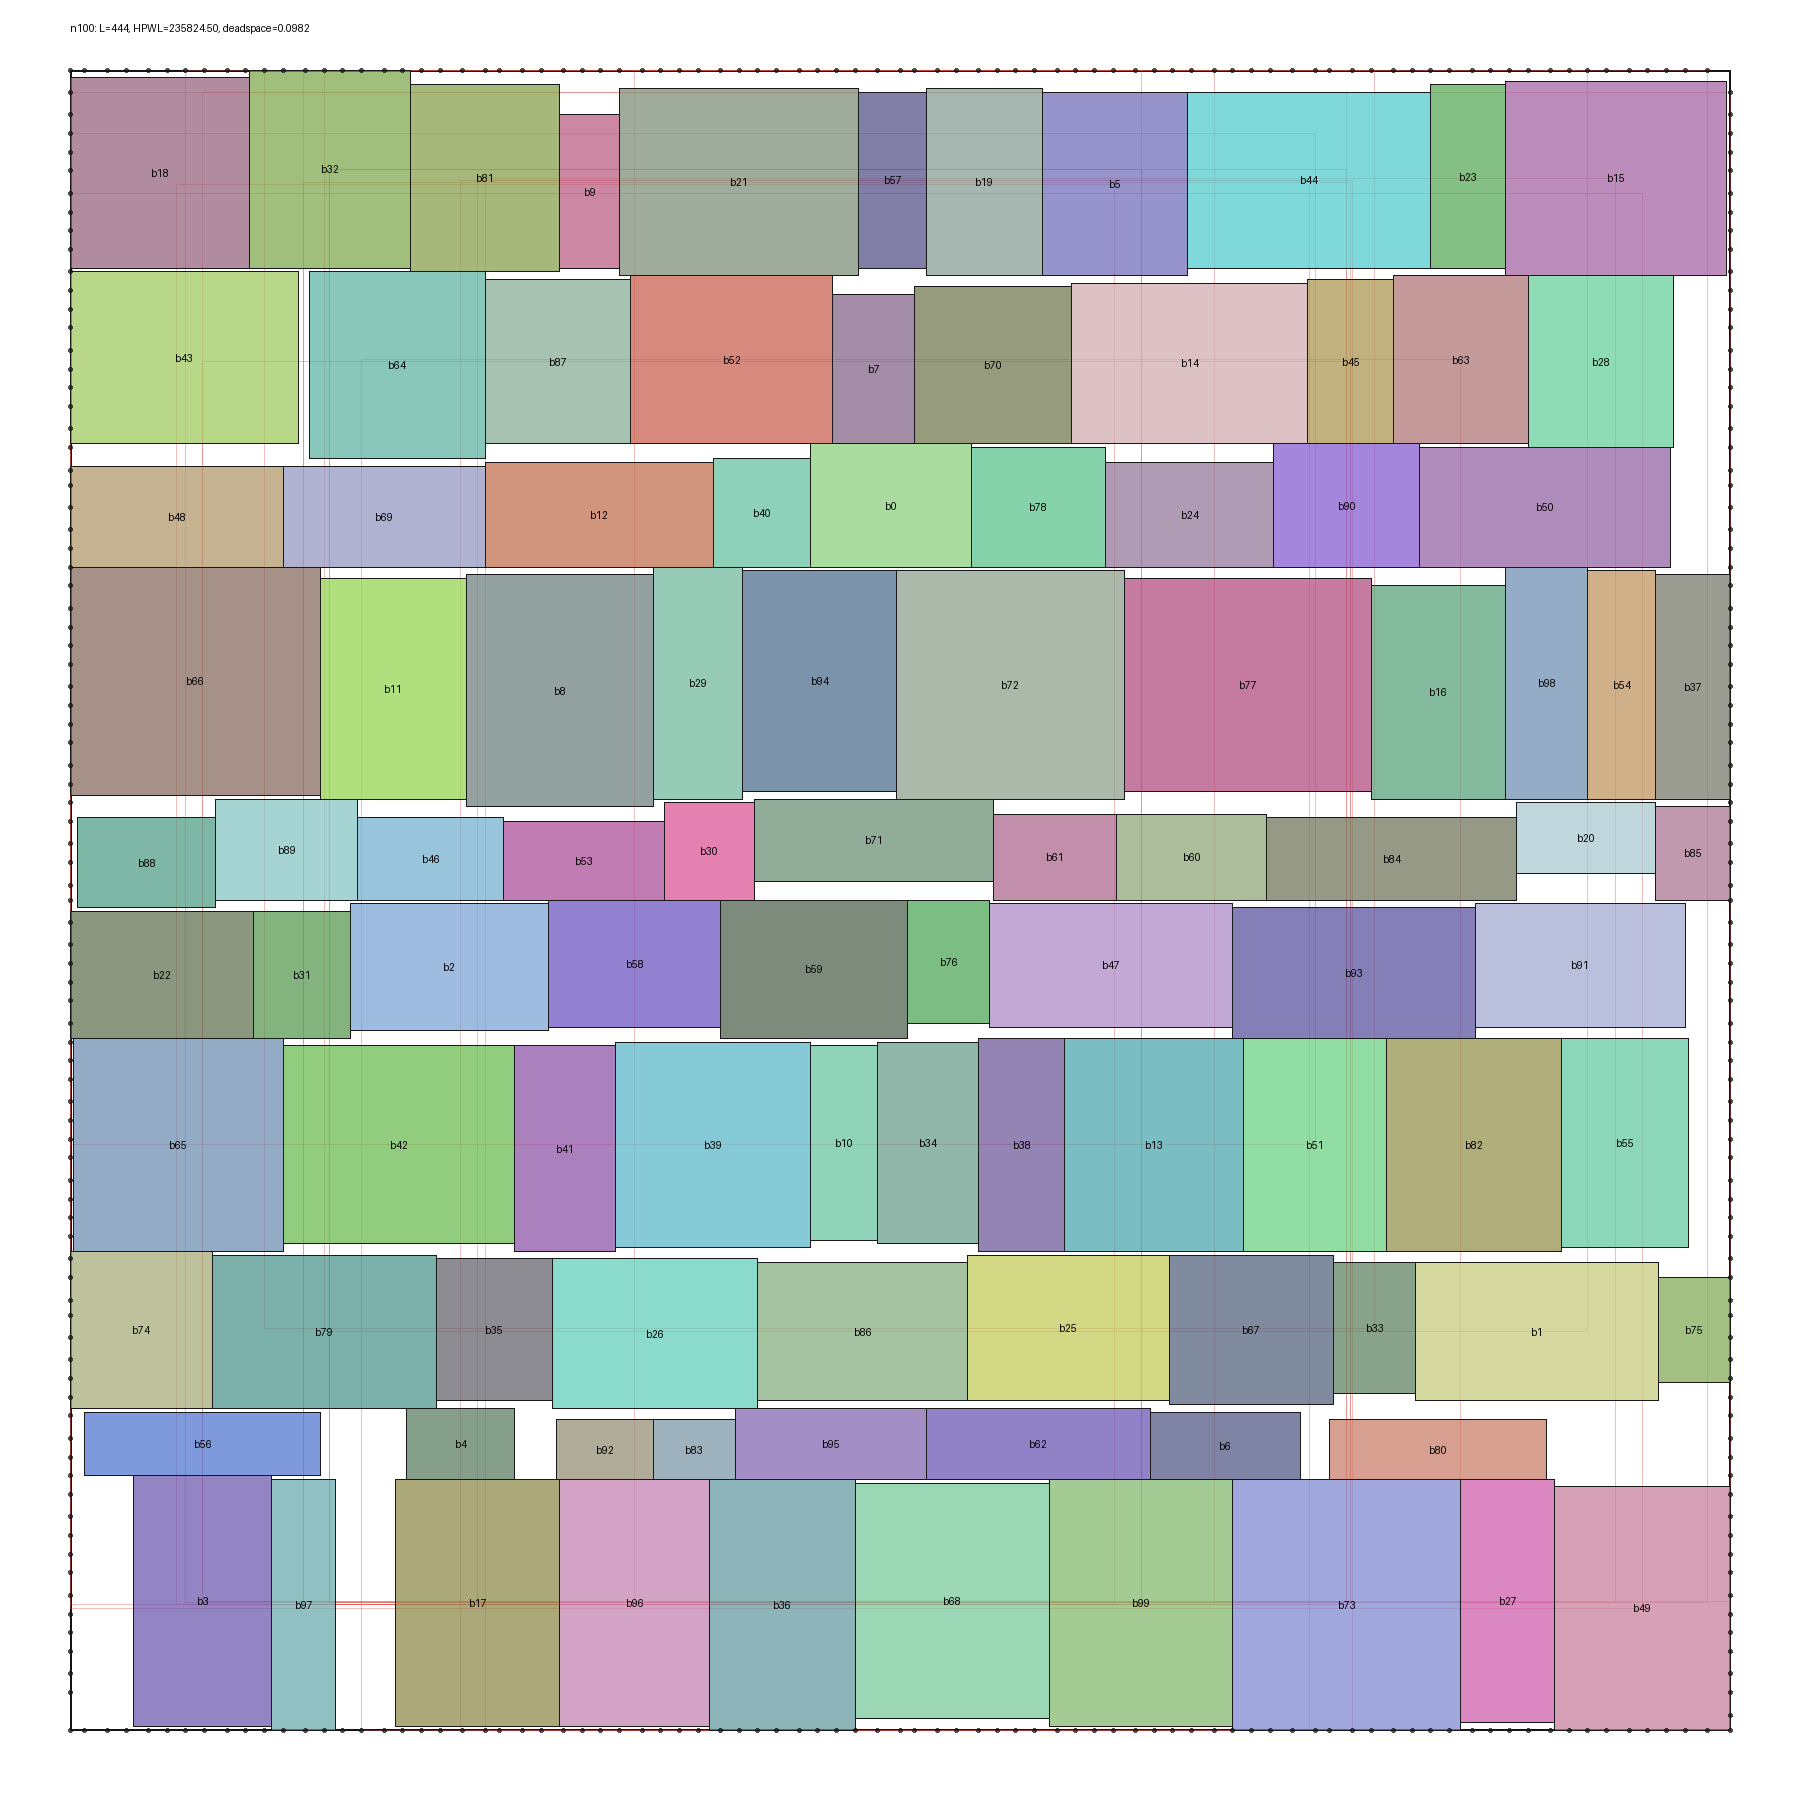
\includegraphics[width=\textwidth]{../results/q3/figures/n100_q3_layout.png}\\[-0.3em]
    {\small (a) \texttt{n100}}
  \end{minipage}
  \hfill
  \begin{minipage}[t]{0.48\textwidth}
    \centering
    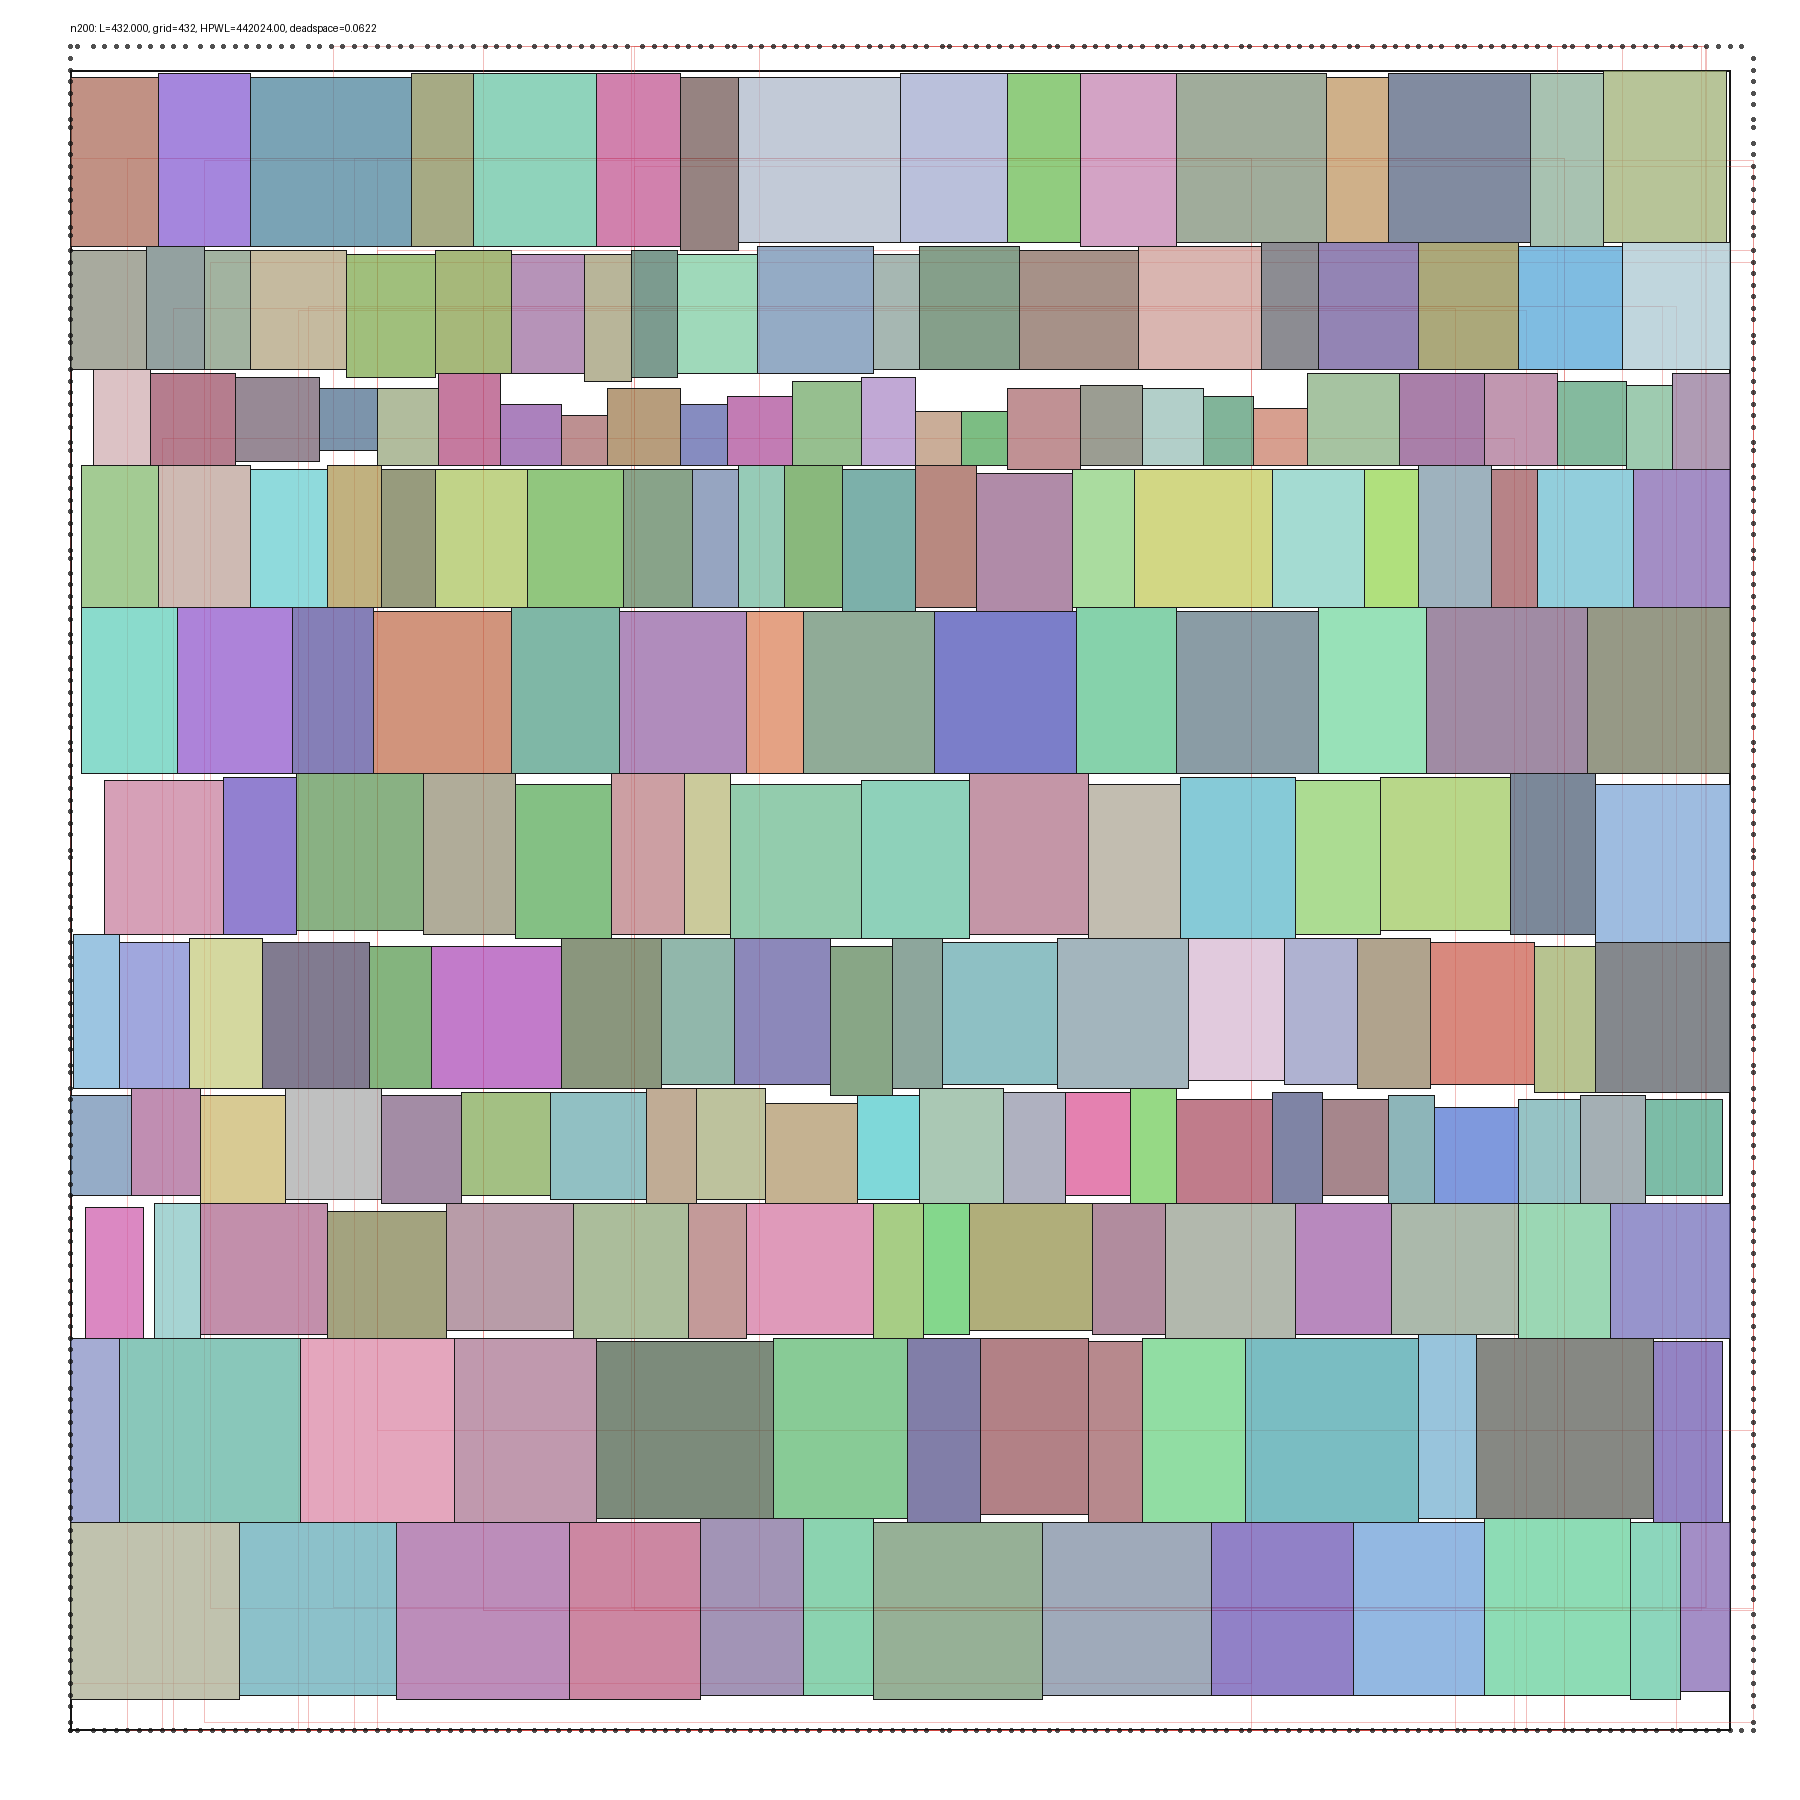
\includegraphics[width=\textwidth]{../results/q3/figures/n200_q3_layout.png}\\[-0.3em]
    {\small (b) \texttt{n200}}
  \end{minipage}
  \caption{问题三 \texttt{n100} 与 \texttt{n200} 的紧轮廓硬模块布局}
  \label{fig:q3_n100_n200}
\end{figure}

\begin{figure}[H]
  \centering
  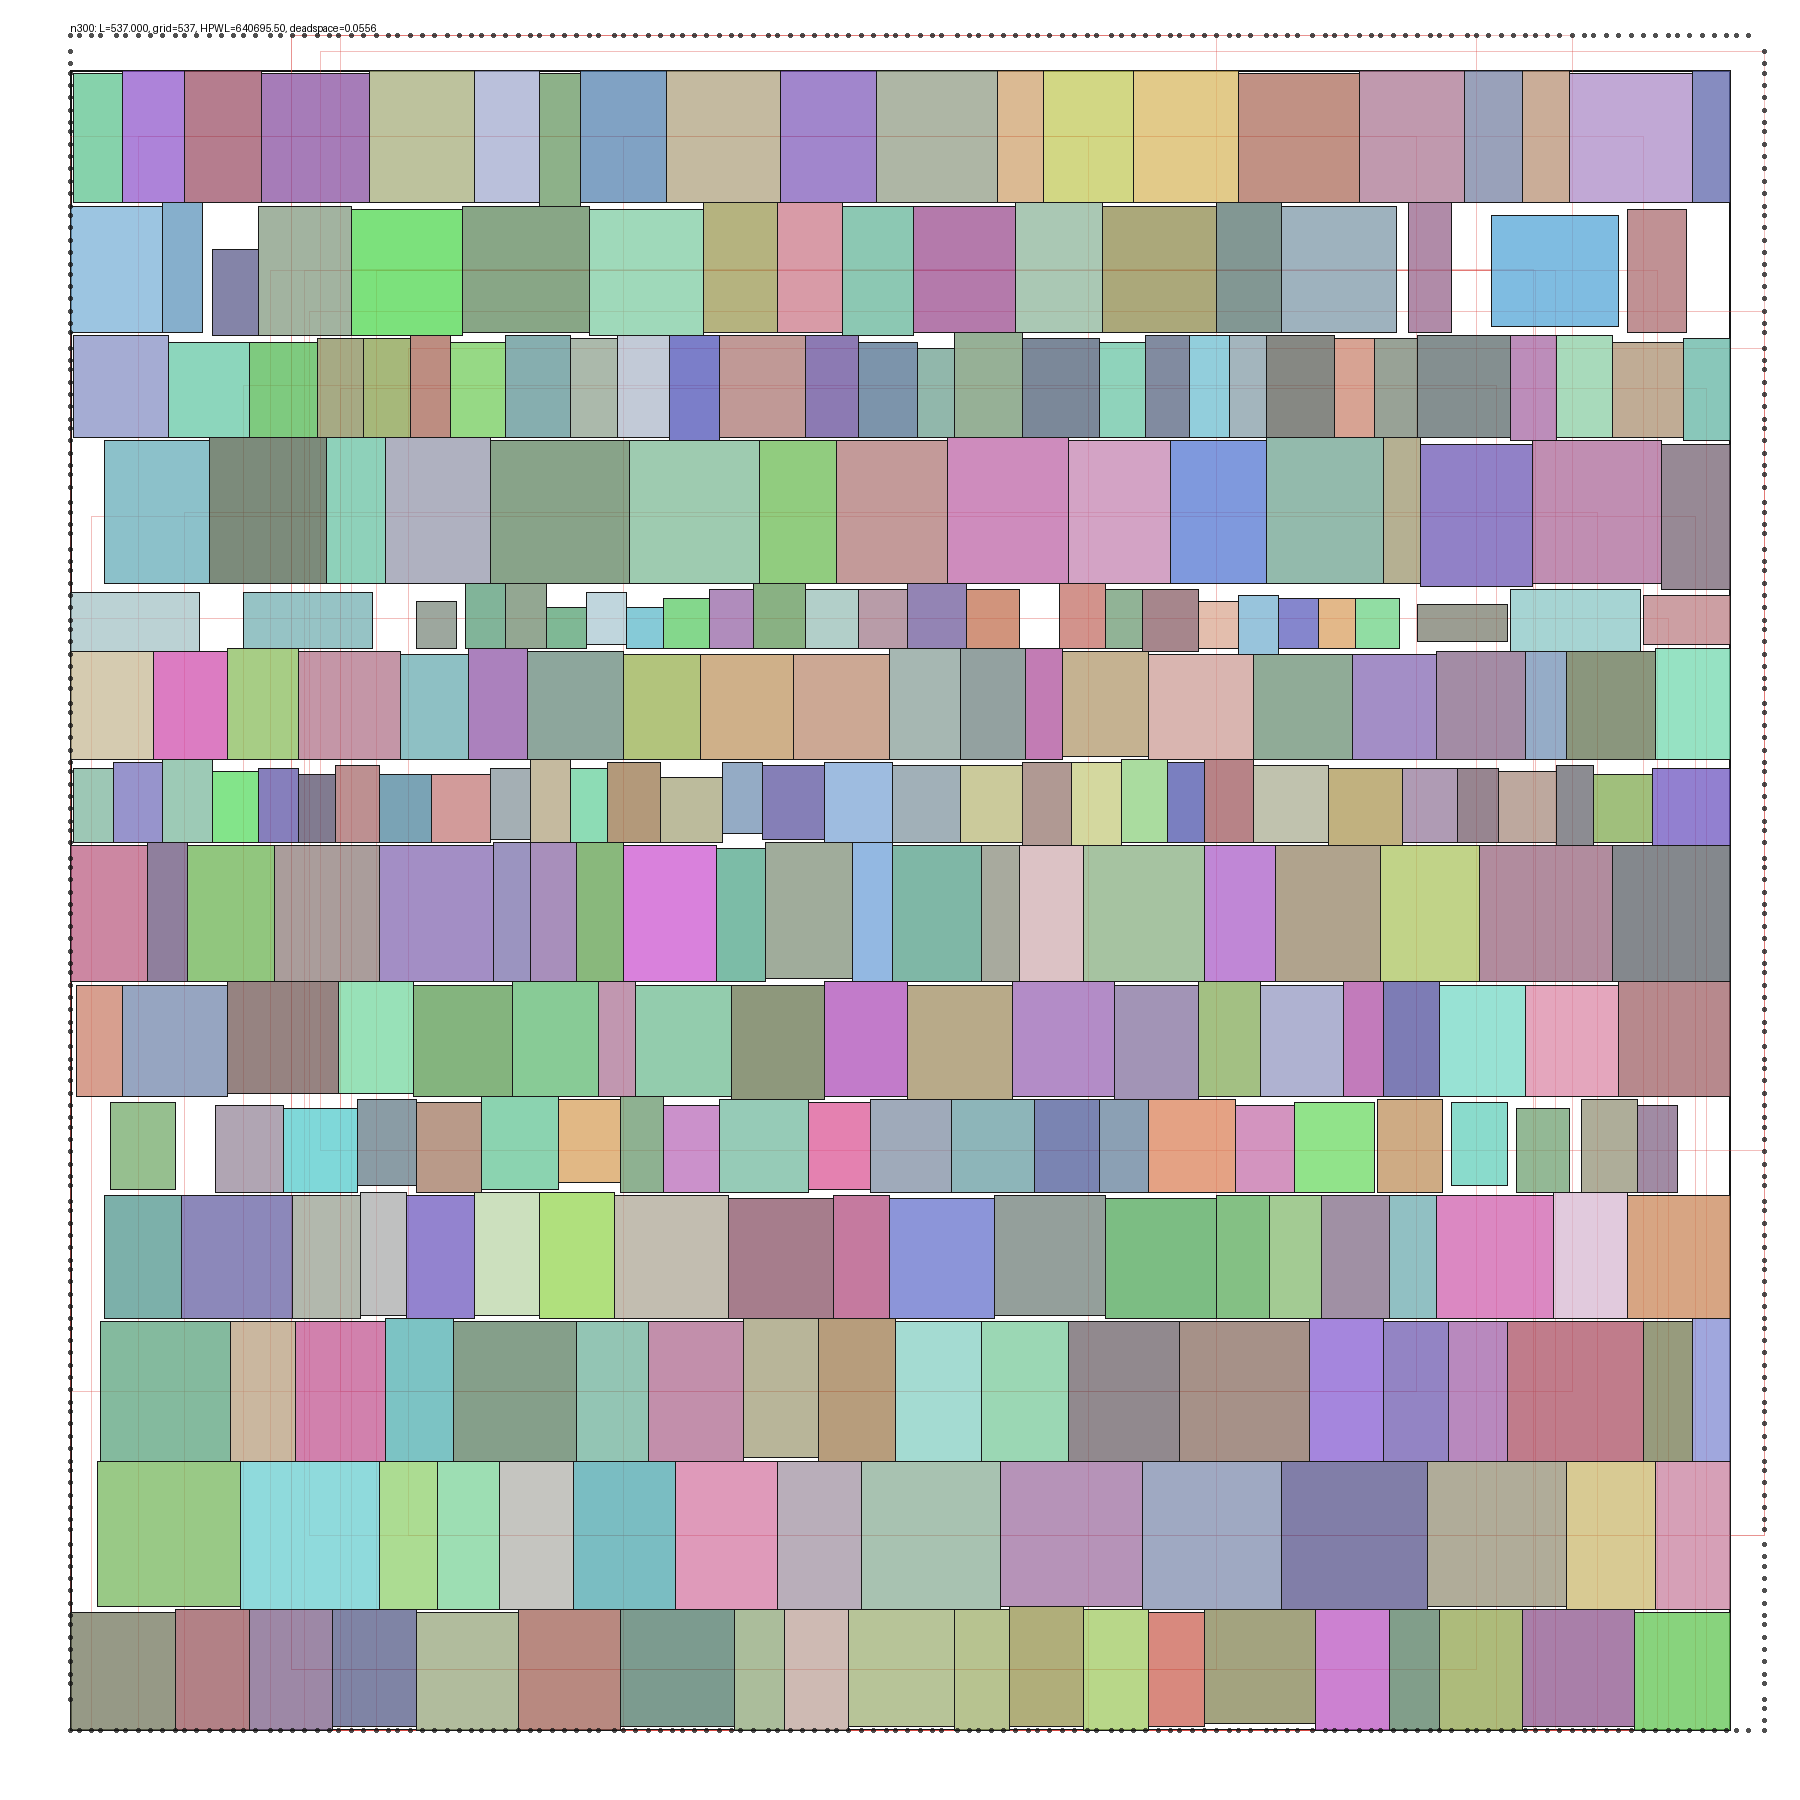
\includegraphics[width=0.76\textwidth]{../results/q3/figures/n300_q3_layout.png}
  \caption{问题三 \texttt{n300} 在边长 $537$、死区率 $5.5639\%$ 下的紧轮廓硬模块布局}
  \label{fig:q3_n300}
\end{figure}

三组布局均在压缩后的正方形内完整摆放全部硬模块。随着轮廓收紧，模块间可交换与可重插入的空间减少，布局图所呈现的高密度结构与图~\ref{fig:q3_tradeoff} 中的 HPWL 增长相互印证。

\subsection{结果检验与本问结论}

程序逐一复核模块名称完整性、轮廓边界、两两非重叠、模块总面积与 HPWL 复算一致性；三组布局均无缺失、重复、越界或重叠，且面积与线长复算结果均与表~\ref{tab:q3_main_results} 一致。完整验证计数及口径敏感性数据见附录 A.2。综上，问题三在保持布局合法的条件下，将死区率由 $15\%$ 显著压缩至 $5.5639\%$--$7.3649\%$，但相应付出了约 $7.79\%$--$14.31\%$ 的互连线长增量，清晰体现了面积利用率与互连代价之间的权衡。

\section{问题四：非矩形模块布局模型的建立与求解}

本问沿着“外接矩形失效---真实形状集合---精确枚举---下界与构造共同证明最优”的主线，将问题一的矩形装箱模型推广到非矩形模块。

\subsection{几何模型：非矩形模块的形状级表示}

\subsubsection{模块形状解释}

问题四将问题一的矩形模块推广为 L 型、T 型等非矩形模块。矩形外接框不能反映凹槽的真实空闲区域，因此需要将每个模块表示为形状集合，并根据真实占用区域判断是否重叠。根据题面图 3 的标注与单位比例，采用表~\ref{tab:q4_shape_data} 所示的单位格解释。

\begin{table}[H]
  \centering
  \caption{图 3 四个模块的形状解释}
  \label{tab:q4_shape_data}
  \small
  \renewcommand{\arraystretch}{1.15}
  \begin{tabular}{c c c r p{6.0cm}}
    \toprule
    模块 & 类型 & 外接尺寸 & 面积 & 实际占用区域 \\
    \midrule
    b1 & T 型 & $4\times4$ & 12 & 上横为 $4\times2$，下竖为 $2\times2$ \\
    b2 & L 型 & $2\times4$ & 6 & 左竖为 $1\times4$，右下为 $1\times2$ \\
    b3 & 矩形 & $2\times1$ & 2 & 两个相邻单位格 \\
    b4 & 矩形 & $1\times4$ & 4 & 四个纵向相邻单位格 \\
    \bottomrule
  \end{tabular}
\end{table}

其中，题面未以独立文字表格给出 b1 的全部竖向尺寸。根据图中与 b3、b4 一致的单位比例，本文将 b1 解释为外接 $4\times4$、上横高度 $2$、下竖高度 $2$ 的 T 型模块。\textbf{最终数值结果依赖该几何解释；若题面尺寸采用其他解释，则需重新定义 b1 的形状集合并重新求解。}

\subsubsection{形状集合、旋转和平移}

设模块 $i$ 在局部坐标系中的实际区域为有限个轴对齐小矩形的并
\begin{equation}
  \mathcal{S}_i=\bigcup_{k=1}^{m_i}R_{ik}.
  \label{eq:q4_rectangle_union}
\end{equation}
对于图 3 的整数单位格算例，可等价表示为
\begin{equation}
  \mathcal{S}_i
  =\bigcup_{(u,v)\in C_i}[u,u+1]\times[v,v+1],
  \label{eq:q4_cell_shape}
\end{equation}
其中 $C_i$ 是模块 $i$ 的局部占用格集合。旋转角满足
$\theta_i\in\{0^\circ,90^\circ,180^\circ,270^\circ\}$。对 $C_i$ 旋转后重新平移，使其最小横、纵坐标均为 $0$，得到归一化集合 $C_i^{(\theta_i)}$。模块左下角平移至 $(x_i,y_i)$ 后，实际占用格为
\begin{equation}
  \widetilde C_i
  =\left\{(u+x_i,v+y_i):(u,v)\in C_i^{(\theta_i)}\right\}.
  \label{eq:q4_transform}
\end{equation}

\subsubsection{边界、形状级非重叠与面积目标}

设芯片轮廓为 $W\times H$，则每个占用格必须满足
\begin{equation}
  0\le u<W,\qquad 0\le v<H,
  \qquad \forall (u,v)\in\widetilde C_i.
  \label{eq:q4_boundary}
\end{equation}
任意两个不同模块的真实占用格集合必须不交：
\begin{equation}
  \widetilde C_i\cap\widetilde C_j=\varnothing,
  \qquad \forall i<j.
  \label{eq:q4_nonoverlap}
\end{equation}
式~(\ref{eq:q4_nonoverlap}) 允许模块边界接触，也允许一个模块进入另一非矩形模块外接框的凹槽，只禁止实际面积重叠。这是相对问题一矩形模型的核心修正。

对归一化布局，所有模块最小外接轮廓的宽高可由占用格坐标确定：
\begin{equation}
  W=1+\max_{i,(u,v)\in\widetilde C_i}u,
  \qquad
  H=1+\max_{i,(u,v)\in\widetilde C_i}v.
  \label{eq:q4_outline}
\end{equation}
本问仍以外接面积最小为目标：
\begin{equation}
  \min A_{\mathrm{outline}}=WH,
  \quad
  \text{s.t. 式~(\ref{eq:q4_boundary}) 和式~(\ref{eq:q4_nonoverlap})成立}.
  \label{eq:q4_model}
\end{equation}
全部模块的实际面积和为
\begin{equation}
  A_{\mathrm{sum}}=\sum_i|C_i|=12+6+2+4=24.
  \label{eq:q4_total_area}
\end{equation}
任何包围全部模块的轮廓都满足
\begin{equation}
  A_{\mathrm{outline}}\ge A_{\mathrm{sum}}=24,
  \label{eq:q4_area_lb}
\end{equation}
该下界将用于判断枚举所得布局是否达到全局最小面积。

\subsection{求解方法：形状级表示与回溯枚举}

\subsubsection{矩形算法的形状级改造}

问题四并未改变问题一“以外接轮廓面积为目标”的优化任务，改变的是决定可行域与轮廓的几何内核。两种模型在四个关键层面的差异见表~\ref{tab:q4_algorithm_changes}。

\begin{table}[H]
  \centering
  \caption{从问题一矩形模型到问题四形状级模型的四层改造}
  \label{tab:q4_algorithm_changes}
  \small
  \renewcommand{\arraystretch}{1.15}
  \begin{tabular}{p{2.3cm} p{4.2cm} p{6.0cm}}
    \toprule
    算法环节 & 问题一矩形模型 & 问题四形状级模型 \\
    \midrule
    几何表示 & 以宽、高描述单个实心矩形 & 以单位格集合或轴对齐矩形并描述真实占用区域 \\
    旋转状态 & 矩形仅需 $0^\circ$、$90^\circ$ & 生成 $0^\circ$、$90^\circ$、$180^\circ$、$270^\circ$ 并删除重复形态 \\
    重叠检测 & 用矩形方向分离条件判断 & 要求平移后的真实占用集合交集为空，凹槽仍可利用 \\
    轮廓计算 & 对各模块矩形外接框取总外接框 & 对全部真实占用区域直接取最小外接框 \\
    \bottomrule
  \end{tabular}
\end{table}

\subsubsection{四模块回溯搜索}

图 3 只有四个整数尺寸模块。本文先生成每个模块互不重复的四向旋转形态，再按候选轮廓面积递增的顺序枚举 $W\times H$；对固定轮廓，回溯枚举各模块的旋转状态与整数位置，仅保留满足边界约束和真实形状集合不交约束的分支。旋转、位置与候选轮廓均属于有限集合，因此该过程构成完整有限枚举，适合本问的小规模实例。对于大规模非矩形模块，可保留问题一的启发式外层搜索，但几何内核仍须使用形状级相交检测。

\subsection{求解结果与分析}

\subsubsection{最优布局求解结果}

完整枚举得到一个宽 $6$、高 $4$ 的可行布局。具体坐标与旋转状态见表~\ref{tab:q4_placement}，旋转角均以图 3 原始方向为基准顺时针计量。

\begin{table}[H]
  \centering
  \caption{问题四四模块最优摆放方案}
  \label{tab:q4_placement}
  \small
  \renewcommand{\arraystretch}{1.15}
  \begin{tabular}{c r r r c r}
    \toprule
    模块 & $x$ & $y$ & 旋转角/度 & 旋转后外接尺寸 & 面积 \\
    \midrule
    b1 & 1 & 0 & 0  & $4\times4$ & 12 \\
    b2 & 0 & 0 & 0  & $2\times4$ & 6 \\
    b3 & 4 & 0 & 90 & $1\times2$ & 2 \\
    b4 & 5 & 0 & 0  & $1\times4$ & 4 \\
    \bottomrule
  \end{tabular}
\end{table}

由表~\ref{tab:q4_placement} 可构造图~\ref{fig:q4_optimal_layout} 所示的 $6\times4$ 布局，其轮廓面积为
\[
  A_{\mathrm{outline}}=6\times4=24,
\]
而任意可行轮廓必须覆盖全部模块，故均有
\[
  A_{\mathrm{outline}}\ge A_{\mathrm{sum}}=24.
\]
当前具体构造达到等号，因此最小轮廓面积严格为 $24$，死区面积为 $0$。这一全局最优结论来自\textbf{理论下界与具体可行构造}的共同证明，而非单纯的数值搜索。

\subsubsection{形状空间利用分析}

为解释等号为何能够达到，图~\ref{fig:q4_optimal_layout} 用虚线标出 b1 的 $4\times4$ 矩形外接框，并保留四个模块的真实占用形状。

\begin{figure}[H]
  \centering
  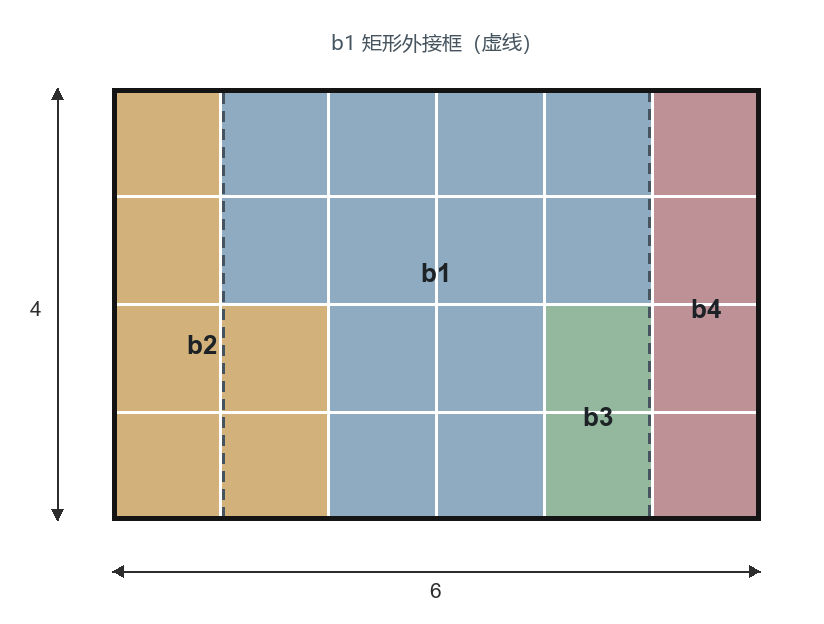
\includegraphics[width=0.76\textwidth]{../results/q4/figures/q4_optimal_layout.png}
  \caption{四个模块利用 b1 凹槽形成的 $6\times4$ 全局最优形状级布局}
  \label{fig:q4_optimal_layout}
\end{figure}

图中，b2 的右下短臂进入 b1 外接框左下方未被 T 型实体占据的凹槽，旋转 $90^\circ$ 的 b3 则进入其右下凹槽；最终真实占用区域均位于轮廓内且两两不交。由此可见，形状级碰撞判定能够利用非矩形模块的凹槽空间，而矩形外接框模型会错误排除这一零死区布局。

因此，本问通过真实形状集合建模利用凹槽，并以“面积下界 $24$ + 面积为 $24$ 的具体构造”严格证明了 $6\times4$ 布局的全局最优性。

\section{敏感性分析与稳健性检验}

由于本文研究的布图规划问题属于离散几何优化，轮廓边长、模块位置与旋转状态的变化通常引起指标的离散响应。因此，本节不对整数决策变量作微分意义下的局部敏感度分析，而是围绕轮廓边长扰动、Terminal 边界口径和跨实例结果一致性进行检验，以判断主要结论是否依赖于个别参数或单一算例。

\subsection{敏感性分析}

\subsubsection{轮廓边长扰动}

由式~\eqref{eq:q3_deadspace}可知，在硬模块总面积 $A_{\mathrm{block}}$ 不变时，死区率 $\Gamma(S)$ 随正方形轮廓边长 $S$ 严格单调增加。以问题三获得的当前最小成功构造边长 $S_{\mathrm{found}}$ 为中心，分别计算 $S_{\mathrm{found}}-1$、$S_{\mathrm{found}}$ 与 $S_{\mathrm{found}}+1$ 对应的理论死区率，结果见表~\ref{tab:sensitivity_side}。

\begin{table}[H]
  \centering
  \caption{轮廓边长扰动下的理论死区率}
  \label{tab:sensitivity_side}
  \small
  \renewcommand{\arraystretch}{1.15}
  \begin{tabular}{c r r r}
    \toprule
    实例 & $\Gamma(S_{\mathrm{found}}-1)$/\% & $\Gamma(S_{\mathrm{found}})$/\% & $\Gamma(S_{\mathrm{found}}+1)$/\% \\
    \midrule
    \texttt{n100} & 6.8763 & 7.3649 & 7.8546 \\
    \texttt{n200} & 5.7286 & 6.2198 & 6.7122 \\
    \texttt{n300} & 5.1711 & 5.5639 & 5.9575 \\
    \bottomrule
  \end{tabular}
\end{table}

表中 $S_{\mathrm{found}}-1$ 对应的数值仅用于衡量目标函数的变化幅度，并不表明该边长下必然存在可行布局。边长增加 $1$ 个单位时，三组实例的死区率分别增加约 $0.49$、$0.49$ 和 $0.39$ 个百分点，变化方向与理论单调性完全一致，不会因数值舍入造成相邻整数边长的目标排序反转。

三组实例的理论搜索下界为 $424$、$420$、$523$，而 $S_{\mathrm{found}}$ 为 $439$、$432$、$537$，分别高出 $15$、$12$、$14$ 个单位，相对差距仅为 $3.54\%$、$2.86\%$、$2.68\%$。这表明当前方案均已进入面积下界附近的紧轮廓区域；但 MaxRects 仍是启发式构造器，上述差距不能作为 $S_{\mathrm{found}}$ 全局最优的证明。

\subsubsection{Terminal 边界口径}

正文将芯片轮廓解释为硬模块的摆放边界，固定 Terminal 仅参与 HPWL 计算。若采用更严格的替代口径，要求所有 Terminal 也位于正方形轮廓内，则根据 Terminal 坐标范围，\texttt{n100}、\texttt{n200} 和 \texttt{n300} 的边长至少需要增至 $444$、$438$ 和 $548$。相对主模型边长分别增加 $5$、$6$ 和 $11$ 个单位，对应死区率为
\begin{equation}
  9.8245\%,\qquad 9.1909\%,\qquad 9.9330\%.
  \label{eq:terminal_sensitivity}
\end{equation}
较主模型结果分别上升 $2.46$、$2.97$ 和 $4.37$ 个百分点。因此，Terminal 是否受轮廓约束会对问题三的死区率数值产生明显影响，是本题中需要明确的重要边界口径。

即便采用该替代口径，三组死区率仍均低于问题二设定的 $15\%$，因而“收紧轮廓能够提高面积利用率”的主要结论不受题意解释改变。正文保留硬模块轮廓口径，并将替代口径的诊断计数列于附录 A.2。

\subsection{稳健性检验}

\subsubsection{几何可行性与指标复算}

对问题一至问题三的最终布局，程序独立检查模块名称完整性、轮廓边界、两两非重叠、模块总面积和 HPWL 复算一致性。三组实例均未出现模块缺失、重复、越界或重叠，面积与线长复算结果也与正文表格一致。因此，尽管大规模组合优化采用启发式算法，不具有全局最优性保证，所得坐标方案仍可确认为满足原模型几何约束与指标口径的合法可行解。

问题四则具有更强的最优性证据：四个模块的实际面积之和为 $24$，任意可行外接轮廓的面积不小于 $24$；完整有限枚举又成功构造出面积恰为 $24$ 的 $6\times4$ 布局。因此，该结果由理论下界与可行构造共同证明为全局最优。

\subsubsection{跨实例变化规律}

在问题二中，局部重插入使 \texttt{n100}、\texttt{n200} 和 \texttt{n300} 的 HPWL 分别降低 $1.7809\%$、$0.3709\%$ 和 $0.6185\%$。三组实例的改善幅度不同，但变化方向一致，说明“网络驱动目标位置---几何合法化---局部重插入”的分层流程能够在不破坏几何可行性的前提下，稳定回收合法化阶段造成的部分线长损失。

在问题三中，三组实例的死区率均由 $15\%$ 降至 $5.5639\%$--$7.3649\%$，同时 HPWL 较问题二分别增加 $8.7489\%$、$7.7917\%$ 和 $14.3094\%$。不同规模网表均呈现“轮廓收紧---线长增加”的同向规律，说明该权衡并非单一算例的偶然结果，而与紧轮廓减少模块位置调整空间的机制相一致。

综合上述检验，本文方案在几何约束、指标复算与跨实例变化规律三个层面均具有一致性。Terminal 边界口径虽会改变问题三的具体死区率，但不会改变轮廓收紧能够提高面积利用率，以及面积利用率与互连线长之间存在权衡的核心结论。

\section{模型评价与推广}

\subsection{模型优点}
\begin{enumerate}[label=\arabic*.,leftmargin=2.4em,itemsep=0.35em]
  \item \textbf{模型体系统一且递进。}本文以模块旋转、坐标和非重叠关系为共同几何基础，从自由轮廓依次扩展至固定轮廓与网络线长、紧轮廓搜索，再将矩形表示推广至非矩形的真实占用区域集合。四个问题可复用共同的变量、约束与检验逻辑，同时保留各问的特有目标。
  \item \textbf{优化层级与题目目标一致。}问题一对外接面积和轮廓长短边比采用词典序判优，问题三则以“先压缩轮廓、再优化 HPWL”构造词典序目标。这一处理不需要人为设定面积与线长的加权系数，避免了额外权重对目标优先级的改变。
  \item \textbf{网络信息与离散几何约束分层处理。}问题二先由二次线长松弛提取网络驱动的目标位置，再进行几何合法化和局部重插入。这一流程将网络引导与几何可行性分工，缓解了位置、旋转、非重叠与 HPWL 在高维离散空间中直接联合搜索的困难。
  \item \textbf{结果具有可复现的证据链。}问题一至问题三均输出模块坐标、旋转状态与布局图，并独立复核完整性、边界、非重叠与目标函数；问题四进一步以理论面积下界和具体可行构造闭合最优性证明，使数值结果与结论强度保持匹配。
  \item \textbf{形状级几何表示能够利用非矩形凹槽。}问题四不以外接矩形代替 L 型、T 型模块，而依据真实占用集合判断碰撞，因而允许其他模块进入未被实体占用的凹槽。最终零死区布局说明，该表示能够避免外接矩形近似引起的虚假空间占用。
\end{enumerate}

\subsection{模型局限}
\begin{enumerate}[label=\arabic*.,leftmargin=2.4em,itemsep=0.35em]
  \item \textbf{大规模实例尚无法证明全局最优。}问题一的 Skyline 与 MaxRects 构造、问题二的目标引导合法化与局部重插入，以及问题三以 MaxRects 进行的当前轮廓可行构造，均只探索了组合空间的一部分。因此，相应面积、HPWL 和成功构造边长应解释为当前策略与搜索预算下的经验证可行上界，而非严格全局最优值。
  \item \textbf{HPWL 仅是实际互连代价的近似。}HPWL 能以较低代价衡量网络的几何展布范围，是 VLSI 物理设计中常用的线长估计指标~\cite{kahng2011}；但真实布线还受拥塞、障碍、布线层与时序等因素影响，因而较小 HPWL 不必然对应详细布线后的最小实际线长或最小时延。
  \item \textbf{引脚位置采用模块中心近似。}问题二与问题三将硬模块引脚统一置于几何中心。真实宏模块的引脚可能偏离中心且随旋转变化；当模块尺寸较大或引脚集中在某一侧时，中心近似可能改变 HPWL 对位置与旋转状态的评价。
  \item \textbf{问题四的完整枚举难以直接扩展。}当前实例仅含四个模块，旋转与整数位置可以被完整枚举。随着模块数量、轮廓尺度和形状复杂度增长，组合数量将迅速扩张，需要引入具备形状级碰撞检测的启发式或元启发式搜索。
  \item \textbf{部分结果依赖题意边界口径。}Terminal 是否必须位于芯片轮廓内，会改变问题三报告的死区率。本文的敏感性分析表明，该差异不改变主要结论；但在工程应用中，仍需根据芯片 I/O、固定宏单元与封装约束明确边界定义。
\end{enumerate}

\subsection{模型推广}
\begin{enumerate}[label=\arabic*.,leftmargin=2.4em,itemsep=0.35em]
  \item \textbf{引入结构化布图编码以扩大全局搜索范围。}对大规模矩形模块，可进一步采用 Sequence-Pair~\cite{murata1996} 或 B$^*$-Tree~\cite{chang2000} 等非切片布图表示，并结合模拟退火、多起点搜索或混合整数规划。相对单纯的顺序构造，结构化编码能显式表示模块间的相对位置，为更广泛的邻域搜索提供基础。
  \item \textbf{从单一 HPWL 扩展至多物理指标协同优化。}实际 VLSI 物理设计还需同时考虑拥塞、关键路径时延、功耗和热分布等指标~\cite{kahng2011}，可建立
  \begin{equation}
    \min\left(A,\mathcal{L}_{\mathrm{HPWL}},C_{\mathrm{congestion}},T_{\mathrm{delay}},P\right)
  \end{equation}
  的多目标模型。当各指标不存在严格优先关系时，可用 Pareto 前沿代替本文的词典序判优，为设计者提供面积、线长与性能之间的多种折中方案。
  \item \textbf{引入真实引脚位置与网络权重。}若能获得模块内部引脚的局部坐标，可将其随模块平移和旋转同步变换；同时依据时序关键程度设置网络权重，将普通 HPWL 推广为加权 HPWL，以提高模型与后续详细布局及布线代价的一致性。
  \item \textbf{推广至一般直角多边形模块。}对更复杂的 L 型、T 型与一般 rectilinear 模块，可继续以有限矩形并或多边形表示真实占用区域，并将形状级相交判定嵌入 B$^*$-Tree 等全局搜索结构中，使问题四的几何思想不再局限于整数单位格。
  \item \textbf{面向超大规模网表进行分层与并行优化。}当模块数量进一步增长时，可先按网络连接强度将模块聚类为超节点，完成粗粒度全局区域划分，再在各区域内进行精细布局；不同候选轮廓、模块顺序和局部搜索过程也可并行执行，以提高现有分层优化框架对更大规模实例的处理能力。
\end{enumerate}


\clearpage
\begin{thebibliography}{99}
  \sloppy
  \bibitem{kahng2011}
  KAHNG A B, LIENIG J, MARKOV I L, et al. \textit{VLSI Physical Design: From Graph Partitioning to Timing Closure}[M]. Dordrecht: Springer, 2011.

  \bibitem{wong1989}
  WONG D F, LIU C L. Floorplan design of VLSI circuits[J]. \textit{Algorithmica}, 1989, 4(1--4): 263--291.

  \bibitem{murata1996}
  MURATA H, FUJIYOSHI K, NAKATAKE S, et al. VLSI module placement based on rectangle-packing by the sequence-pair[J]. \textit{IEEE Transactions on Computer-Aided Design of Integrated Circuits and Systems}, 1996, 15(12): 1518--1524.

  \bibitem{wei2011}
  WEI L, OON W C, ZHU W, et al. A skyline heuristic for the 2D rectangular packing and strip packing problems[J]. \textit{European Journal of Operational Research}, 2011, 215(2): 337--346.

  \bibitem{jylanki2010}
  JYL\"ANKI J. \textit{A Thousand Ways to Pack the Bin---A Practical Approach to Two-Dimensional Rectangle Bin Packing}[EB/OL]. 2010.

  \bibitem{eisenmann1998}
  EISENMANN H, JOHANNES F M. Generic global placement and floorplanning[C]//\textit{Proc. 35th Design Automation Conference}. 1998: 269--274.

  \bibitem{chang2000}
  CHANG Y C, CHANG Y W, WU G M, et al. B$^*$-Trees: a new representation for non-slicing floorplans[C]//\textit{Proceedings of the 37th Design Automation Conference}. 2000: 458--463.
\end{thebibliography}


\clearpage
\section*{附录 A\quad 支撑材料清单}
\addcontentsline{toc}{section}{附录 A 支撑材料清单}

\subsection*{A.1\quad 数据与结果文件}
问题二三组实例的模块、Terminal 与网络规模见表~\ref{tab:appendix_q2_data_scale}。

\begin{table}[H]
  \centering
  \caption{问题二三组实例的数据规模}
  \label{tab:appendix_q2_data_scale}
  \small
  \begin{tabular}{lrrrr}
    \toprule
    实例 & 硬模块数 & 外部 Terminal 数 & 网络数 & 引脚总数 \\
    \midrule
    \texttt{n100} & 100 & 334 & 885  & 1873 \\
    \texttt{n200} & 200 & 564 & 1585 & 3599 \\
    \texttt{n300} & 300 & 569 & 1893 & 4358 \\
    \bottomrule
  \end{tabular}
\end{table}

\subsection*{A.2\quad 问题三验证与口径敏感性}
问题三完整验证结果见表~\ref{tab:q3_validation_appendix}。其中，轮廓外 Terminal 数与 $S_{\mathrm{terminal}}$ 仅用于检验另一种题意解释：若要求 Terminal 也必须包含在轮廓内，则轮廓边长至少分别为 $444$、$438$、$548$；该替代口径不改变正文采用的硬模块轮廓模型及其结果。

\begin{table}[H]
  \centering
  \caption{问题三布局完整验证与 Terminal 口径敏感性}
  \label{tab:q3_validation_appendix}
  \small
  \renewcommand{\arraystretch}{1.15}
  \begin{tabular}{c r r c c r r}
    \toprule
    实例 & 越界模块数 & 重叠对数 & 面积一致性 & HPWL 复算一致 & 轮廓外 Terminal 数 & $S_{\mathrm{terminal}}$ \\
    \midrule
    \texttt{n100} & 0 & 0 & 是 & 是 & 168 & 444 \\
    \texttt{n200} & 0 & 0 & 是 & 是 & 284 & 438 \\
    \texttt{n300} & 0 & 0 & 是 & 是 & 290 & 548 \\
    \bottomrule
  \end{tabular}
\end{table}

\subsection*{A.3\quad 图表与其他支撑材料}
问题二布局的详细约束与数值一致性复核见表~\ref{tab:appendix_q2_validation}。

\begin{table}[H]
  \centering
  \caption{问题二布局约束与 HPWL 一致性验证}
  \label{tab:appendix_q2_validation}
  \small
  \begin{tabular}{lrrrrcc}
    \toprule
    实例 & 缺失数 & 重复数 & 越界数 & 重叠对数 & 面积一致性 & HPWL 计算一致 \\
    \midrule
    \texttt{n100} & 0 & 0 & 0 & 0 & 是 & 是 \\
    \texttt{n200} & 0 & 0 & 0 & 0 & 是 & 是 \\
    \texttt{n300} & 0 & 0 & 0 & 0 & 是 & 是 \\
    \bottomrule
  \end{tabular}
\end{table}

\section*{附录 B\quad 程序代码}
\addcontentsline{toc}{section}{附录 B 程序代码}

\subsection*{B.1\quad 运行环境与复现说明}

全部程序使用 Python 3 编写，所需第三方依赖统一列于项目根目录的 \texttt{requirements.txt}。在项目根目录中安装依赖后，依次运行问题一至问题四的主程序，即可在 \texttt{results/q1}—\texttt{results/q4} 目录中重新生成布局坐标、结果汇总、验证记录与布局图。推荐的执行顺序为
\begin{enumerate}[label=\arabic*.,leftmargin=2.4em,itemsep=0.2em]
  \item \texttt{python src/q1\_floorplanning.py}；
  \item \texttt{python src/q1\_layout\_figures.py}；
  \item \texttt{python src/q2\_fixed\_outline\_hpwl.py}；
  \item \texttt{python src/q3\_min\_deadspace.py}；
  \item \texttt{python src/plot\_q3\_tradeoff.py}；
  \item \texttt{python src/q4\_nonrect\_floorplanning.py}。
\end{enumerate}
论文采用 XeLaTeX 排版，在 \texttt{paper} 目录内连续两次执行 \texttt{xelatex main.tex} 即可生成完整 PDF。

\subsection*{B.2\quad 完整程序代码}

鉴于完整求解与绘图程序篇幅较长，本文不在附录中重复排印源码。可提交压缩包已保留 \texttt{src} 目录下的全部 Python 程序，其中：
\begin{itemize}[leftmargin=2.4em,itemsep=0.2em]
  \item \path{src/q1_floorplanning.py} 负责问题一的自由轮廓搜索；
  \item \path{src/q2_fixed_outline_hpwl.py} 负责问题二的网络驱动合法化与局部优化；
  \item \path{src/q3_min_deadspace.py} 负责问题三的整数边长搜索；
  \item \path{src/q4_nonrect_floorplanning.py} 负责问题四的形状级枚举。
\end{itemize}
其余脚本用于生成论文图表。所有最终数值、坐标与验证记录一并保存于 \texttt{results} 目录，便于对照正文复核。


\end{document}
